
% $Id: chapter4.tex 2612 2008-06-03 18:32:54Z jozinke $
%
%%\pagestyle{scrheadings}
%%\ohead[]{}
%%\ihead[]{}
%%\chead[]{}
%%\ofoot[\pagemark]{\pagemark}
%%\ifoot[]{}

\chapter{Evaluation} \label{sec:evaluation}


The following section presents the performance evaluation of the proof of concept \ac{IPS} Simplefail2ban, in conjunction
with the test server. First, an overview over the test environment and the experimental design is given and the Fail2Ban performance
issues, discovered by Florian Mikolajczak, are replicated for the test server. Subsequently, the result for Simplefail2ban in both the logfile
and shared memory based variants are presented. The section concludes with an evaluation of different features of the shared memory implementation. 

\section{Test Environment}

To conduct the evaluation, two machines with an identical hardware and software configuration where used. The specific hardware and software version are listed in Table \ref{tab:specs}.
One machine served as the dut, running the test application, as well as Fail2Ban / Simplefail2ban. The second machine was used for traffic generation with TRex.  

\begin{table}[b!]
	\renewcommand{\arraystretch}{1.5}
	\caption[Testbed Summary]{Hardware and Software parameters for the test environment. The measurements where conducted
	on two identical machines, where one machines served as the \ac{DUT}, running the test application and Fail2Ban / Simplefail2ban,
	while the other generated test traffic with trex.}
	\label{tab:specs}
	 \centering
	\small
	\begin{tabular}{ll}
	\toprule
	\multicolumn{2}{l}{\textbf{Hardware}}                                        \\ \midrule
	CPU      & 16 $\times$ Intel(R) Xeon(R) Silver 4314 CPU @ 2.40GHz \\
	NIC      & Mellanox ConnectX-6 100GbE                       \\
	RAM        & 128GB                                                       \\ \bottomrule
	\multicolumn{2}{l}{\textbf{Software}}                                        \\ \midrule
	OS         & Debian 11                                                  \\
	Kernel          & 6.1.0-0                                                   \\
	NIC Driver & mlx5\_core, 6.1.0-0                                      \\
	Fail2Ban       & 0.11.2                                     \\
	TRex            & 3.02                                       \\ \bottomrule
	\end{tabular}
\end{table}

\section{Experimental Design}

The experimental design is closely oriented at experiment 1 conducted by Florian Mikolajczak in \cite{mikolajczak2022}, in order to provide comparable results.
In the experiment, a \ac{DOS} attack on a server under a normal workload is simulated, through a stream of valid a request and a significantly larger
stream of invalid request. The original experiment used a BIND DNS server as the target of the \ac{DOS} attack, which triggered log messages for clients exceeding a certain rate limit. For   
the following evaluation, the test server introduced in \ref{sec:test_server} will serve at the target, differentiating valid and invalid request by the sent payload\footnote{Request are considered invalid, if the first byte if the payload has the unsigned value 42 (ASCII Letter B)}.
While this way of identifying unwanted request is not necessarily realistic, it is efficient and allows the test application to quickly produce log messages.
\par
The goal of this evaluation is to test, how Simplefail2ban performs for the test scenario described above. 
Following the guidelines proposed by Jain \cite{jain:art} performance metrics and factors were defined and system / workload parameters identified:  


\minisec{Performance Metrics}
\begin{itemize}
	\item Total amount of invalid requests dropped (number of packets)
	\item Total amount of invalid requests dropped, relative to the total amount of invalid
	request sent (percentage)
	\item Amount of log messages processed by Simplefail2ban, relative the amount of log messages
	sent by the test server (percentage)
	\item \ac{CPU} utilization of Simplefail2ban (percentage)
\end{itemize}

\minisec{Parameters}
\begin{itemize}
	\item Hardware and software parameters of the environment listed above (\ref{tab:specs}). Especially:  
	\begin{itemize}
		\item \ac{CPU}: 16 cores, no hyper-threading enabled
		\item \ac{NIC}: MTU 1500 bytes
		\item TRex: One interface, 30 threads
	\end{itemize}
	\item Number of entries in \ac{eBPF} maps for \ac{IPv4} \& \ac{IPv6} : 1000000
	\item Number of receiving threads used by the test server : 16
	\item Duration of the measurement : 300 seconds
	\item Amount of valid traffic sent : 10000 \ac{PPS}
	\item Amount of clients sending valid traffic : 254
	\item Simplefail2ban parameters 
		\begin{itemize}
		\item Number of banning thread used : 4 (shared memory), 1 (logfile)
		\item Number of hash table bins used : 6000011
		\item Ban threshold for clients : 3
		\item Ban time for clients : 30 Seconds
		\item Line count for shared memory buffer segments : 100000
		\item Segment count for shared memory buffer : 16
		\item Buffer size for io\_uring getline : 1024
		\end{itemize}
\end{itemize}

\minisec{Factors \& Levels}
\begin{itemize}
	\item Amount of invalid traffic sent : 100k, 1m, 10m \ac{PPS}
	\item Amount of clients sending invalid traffic : 65534, 131086
	\item IP stack: \ac{IPv4}, \ac{IPv6}, \ac{IPv4} / \ac{IPv6} mixed
	\item Simplefail2ban factors 
	\begin{itemize}
		\item IPC Type: Logfile / Shared Memory
		\item Overwrite / No Overwrite (shared memory only)
		\item 2nd Reader / No 2nd Reader (shared memory only)
		\item Workload stealing / No workload stealing (shared memory only)
		\item \ac{Regex} matching / No \ac{Regex} matching
	\end{itemize}
\end{itemize}

The measurements are conducted with TRex scripts, which define a packet stream, that can be customized to generate traffic
in accordance with the factor levels listed above. The scripts are adapted from the original TRex scripts used by Florian Mikolajczak \cite{mikolajczak2022} 
and can be found in the \texttt{src/scripts/traffic\_gen} directory of the thesis Git repository \cite{gitlab}. 
For measuring traffic rates as well as the number of dropped packets, an adapted version of the \texttt{xdp\_ddos01\_blacklist\_cmdline} program
from the implementation of Florian Mikolajczak was used \cite{mikolajczak2022}. The program repeatedly polls maps
maps that are continuously updated by the loaded \ac{eBPF} program with the number of passed and dropped packets.  
\par
\minisec{Experiment 1: Fail2ban Replication}
The first experiment experiment is a replication measurement, meant to replicate the results obtained by Florian Mikolajczak \cite{mikolajczak2022}
for the new test environment. This is done, in order to verify, that the performance issues persist the new test application
as well as the upgraded hardware, compared to when the experiment was first conducted. Two constant streams of UDP packets will be sent to
the test server, one of which contains invalid payloads that trigger log messages and should eventually result in the banning of the clients. The chosen factor levels are the same as in the 
original experiment, at 50000 valid requests per second and 1000000 invalid request from 254 different clients. The only difference is the reduction of the 
ban time from 180 to 60 seconds and the overall measurement time, from 900 to 300 seconds.
\par
As a variation, a seconds Fail2ban measurement is conducted, which lowers the traffic invalid and valid traffic rates to 10000 \ac{PPS}
but increases the number of clients sending invalid request to 1016. This experiment aims at evaluating the scaling of Fail2bans performance in terms
of the number of clients.
\minisec{Experiment 2: Simplefail2ban Logfile}
Experiment 2 evaluates the performance the logfile-based variant of Simplefail2ban. The setup follows that of Experiment 1, but the parameters 
are instead chosen as listed in the Parameters section above. The factors that a varied are the amount of invalid traffic, the amount of clients 
sending invalid requests and the \ac{IP}-stack used for the \ac{UDP} traffic. Simplefail2ban is used with \ac{Regex} matching enabled. In total, 9 measurement are conducted.    
\minisec{Experiment 3: Simplefail2ban Shared Memory}
Experiment 3 mirrors experiment 2, except that the shared-memory based variant of Simplefail2ban of Simplefail2ban is evaluated. For the
measurement, workload stealing and overwrite are disabled and no second reader is attached to the shared memory ring buffer. Simplefail2ban is used with \ac{Regex} matching enabled In total, 9 measurement are conducted.    
\minisec{Experiment 4: Shared Memory Features}
The final experiment evaluates the different features of the shared memory implementation. All measurements are conducted with the highest load scenario, since performance 
differences are expected to be most pronounced there. Hence, the invalid traffic rate is choses at 10m \ac{PPS}, the amount of clients sending invalid traffic at 131068
with a mixed \ac{IPv4} \& \ac{IPv6} stack. The factors that are varied (individually) are overwrite, adding a second reader, workload stealing and disabling \ac{Regex} matching.
In total, 4 measurements are conducted.    
\par
In the following sections, the results of experiments 1 through 4 are presented.

\pagebreak

\section{Experiment 1: Fail2ban Replication}

\begin{figure}[h!]
    \centerline{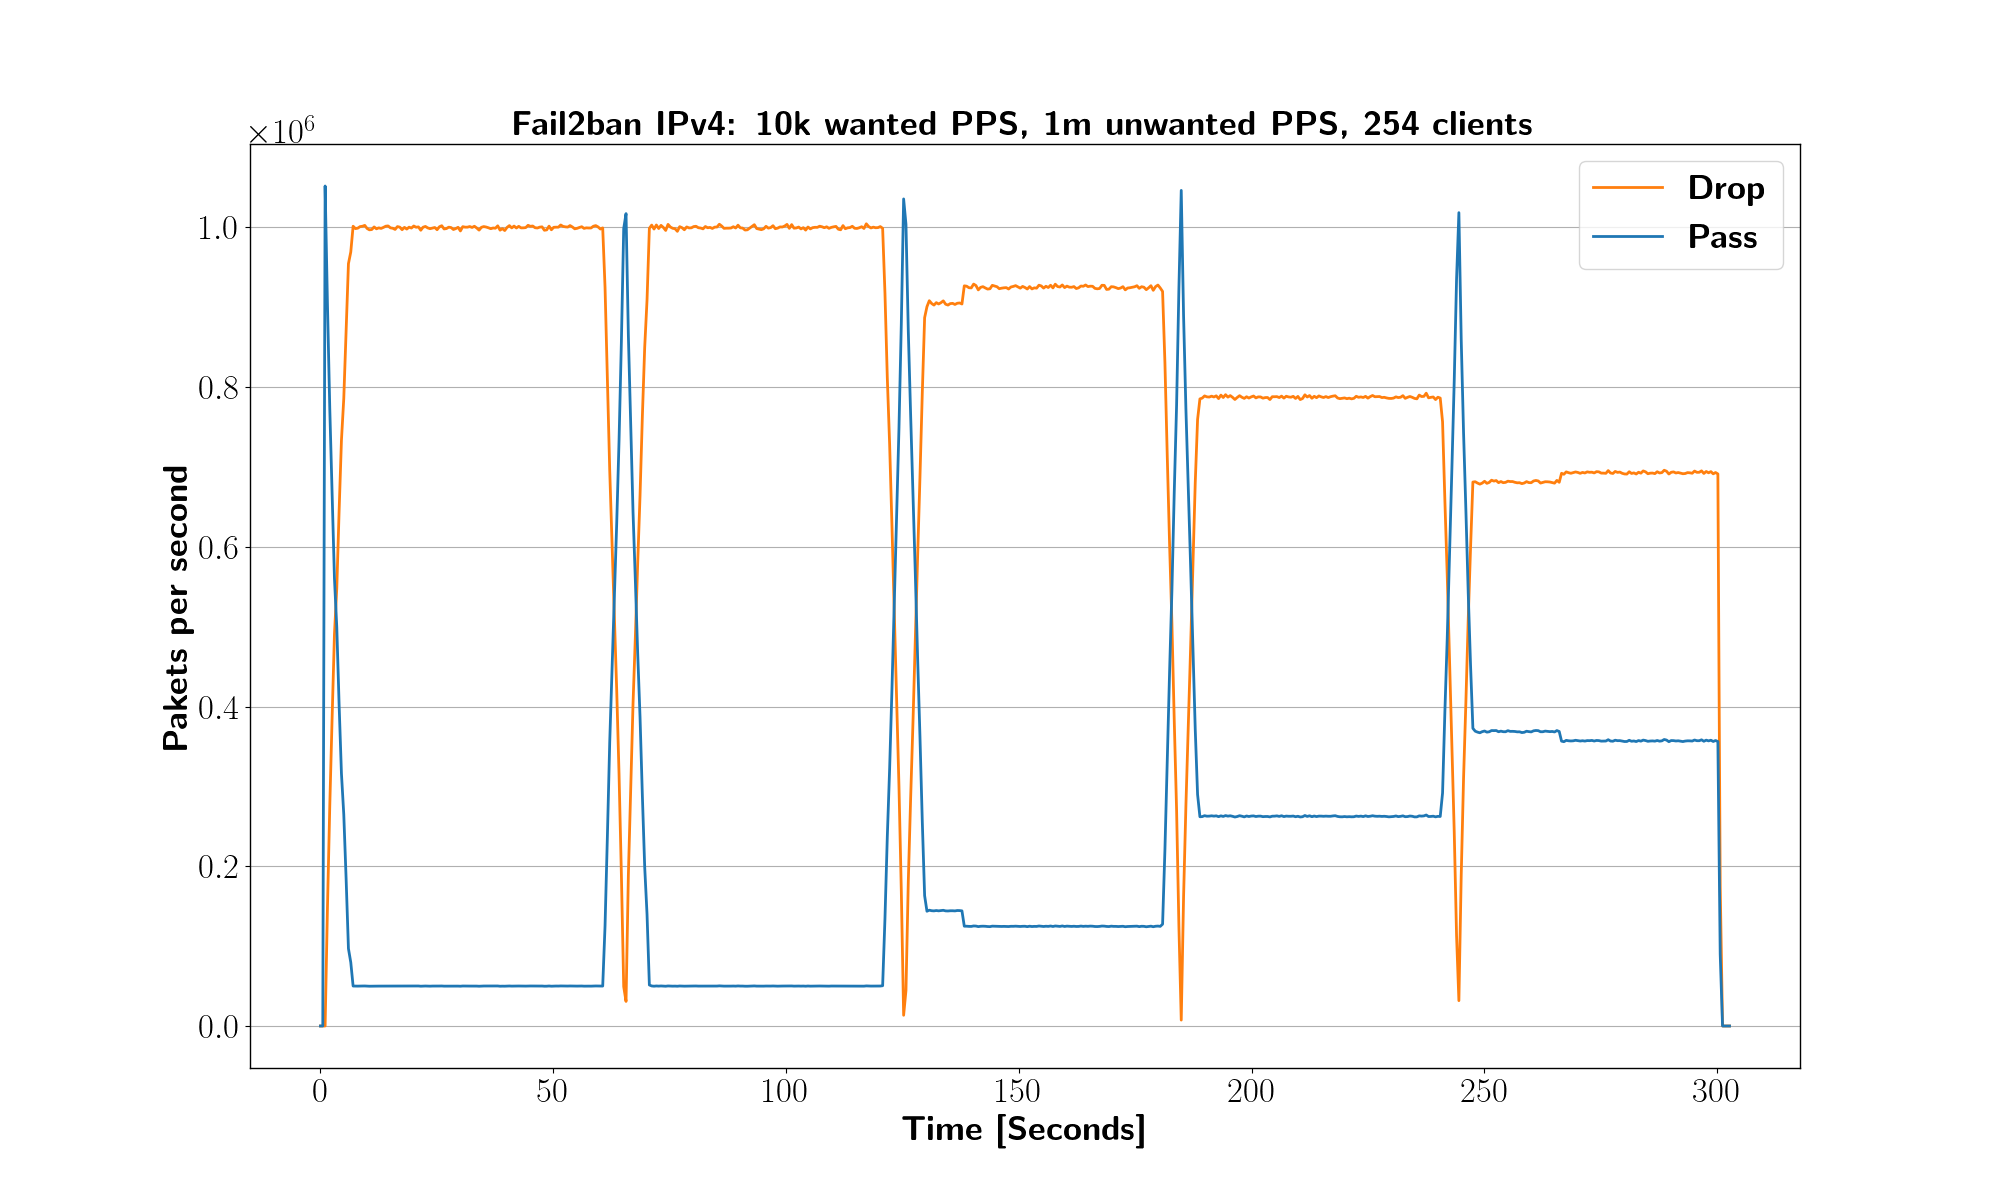
\includegraphics[width=1.2\textwidth]{images/fail2ban_v50k_iv1m_c254.png}}
    \caption[Fail2ban Replication: 1m PPS, 254 Clients]{Fail2ban Replication: 1 million invalid \ac{PPS} from 254 Clients, 50 thousand valid \ac{PPS}}
	\label{fig:fail2ban:1m}
\end{figure}

Figure \ref{fig:fail2ban:1m} displays the results of the replication measurement. While the results differ from those presented in \ref{fig:fail2ban:mikolajczak2022},
a similar pattern can be observed overall. Initially, Fail2ban performs as expected, banning all unwanted traffic for the specified duration. This even holds
for two full ban cycles, which is the first notable differences from previous measurements. After the second ban cycle, the drop rate falls below the expected level and
does not recover after subsequent ban cycles. The reason for this behavior is unclear. One hypothesis in the original work by
Florian Mikolajczak \cite{mikolajczak2022} was, that the initial ban cycle is successful due to TRex slow build up of the traffic rate. However, this does not explain the success
of the second ban cycle, where the traffic rate is at full capacity. Another possible explanation could be, that Fail2bans responsiveness fluctuates due to internal or external factors.
If the responsiveness is low at the end of a ban cycle, Fail2ban does not ban enough clients in time and is overwhelmed by the influx of log messages. However, this remains speculation and warrants
further investigation into Fail2bans performance for future work.
\par
\begin{figure}[h!]
    \centerline{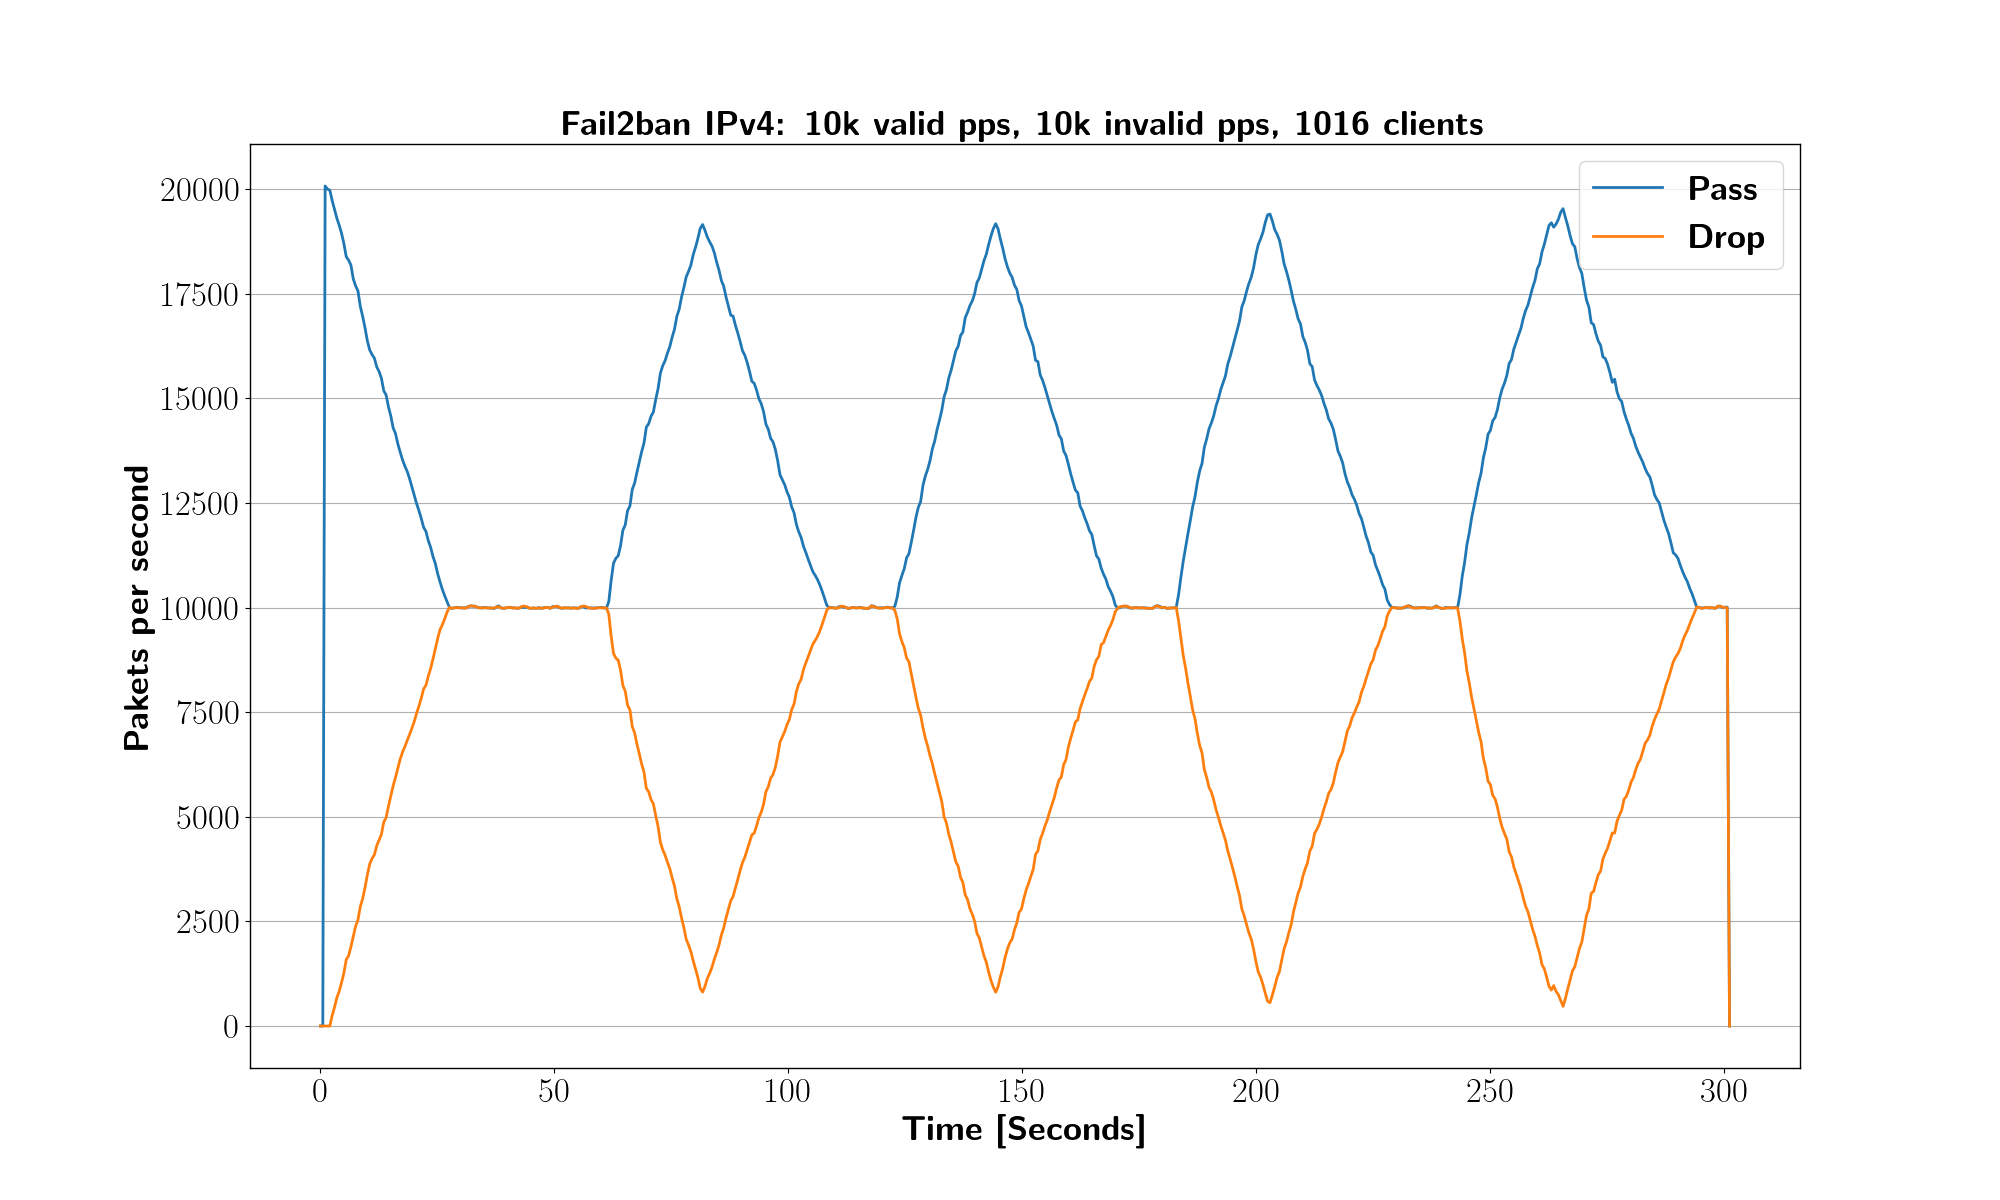
\includegraphics[width=1.2\textwidth]{images/fail2ban_v10k_iv10k_c1016.png}}
    \caption[Fail2Ban Replication: 10k PPS, 1016 Clients]{Fail2ban Replication: 10 thousand invalid \ac{PPS} from 1016 Clients, 10 thousand valid \ac{PPS}}
	\label{fig:fail2ban:10k}
\end{figure}
Figure \ref{fig:fail2ban:10k} presents the results for the second Fail2ban measurement. Here, the result are much more in line with expectation. While Fail2ban manages 
to ban and unban all clients for repeated ban cycles, it takes more than 20 seconds for both banning and unbanning. The measurement was repeated for a smaller number of clients, which
resulted in significantly better performance. This illustrates, that the number of different clients managed by Fail2ban
has a strong impact on the performance of Fail2ban, even at low traffic rates. 
\par 
Overall, the replication managed to show, that Fail2bans performance issues still persist in the new test environment. Both the rate of traffic as well as the number of clients appear
to be significant factors, for which Fail2bans performance scales poorly.  

\pagebreak

\section{Simplefail2ban Measurements}

The following sections present the results for the Simplefail2ban evaluation. To make the reading experience more concise, figures presenting the results 
for the dedicated \ac{IPv4} and \ac{IPv6} measurement have been moved to the annex. However, their results will still be discussed as part of this chapter.

\minisec{Disclaimer}
Upon renewed replication of the measurement, some discrepancies where discovered, which had not been observed when the initial measurements and replication where conducted.
More specifically, the performance measured for Simplefail2ban appears to vary, which is most pronounced for the 10 million \ac{PPS} measurements. On some replication attempts
The unbanning and renewed banning of clients took about 5 to 10 seconds longer than in previous measurement, resulting in a lower rate of dropped packets relative to the expected drop rate.
I have not been able to identify, wether this is caused by a change in the test environment or is simply a characteristic of the implementation. Unfortunately, I lack the time
to conduct a proper variance assessment in time for submission of this thesis. Hence, the disclaimer is issued, that the results presented in the following may not be fully
representative of the average system performance. A more thorough investigation of this problem will be provided at the thesis presentation. \\ 

\minisec{Result overview}
For the \ac{IPv4} and \ac{IPv6} measurements 65534 clients where used for sending invalid traffic,
while the mixed \ac{IPv4} \& \ac{IPv6} measurement was conducted with 131068 clients. The total packets, packets dropped and
log messages colum in the following figures are absolute values, aggregated across the entire measurement time. Total packets refers to the sum of both dropped and passed packets. Log messages refers to the number of messages processed by Simplefail2ban\footnote{For nearly all measurement, this number was the exact same as the number of log messages written by the test server. If not, it will be explicitly stated otherwise.}.
Relative drop refers the number of dropped packets, relative to the ideally expected amount of dropped packets. This number is given by: total dropped packets $/ ($total packets $-$ experiment duration $*$ valid traffic rate $-$ number of ban cycles $*$ ban limit$)$. Finally, \ac{CPU} refers to the \ac{CPU} usage for Simplefail2ban
during the entire measurement, as given by top. 

\subsection{Experiment 2: Logfile Variant}

\begin{figure}[!h]
	\centering
	\scriptsize
	\begin{tabular}{c}
    	\centerline{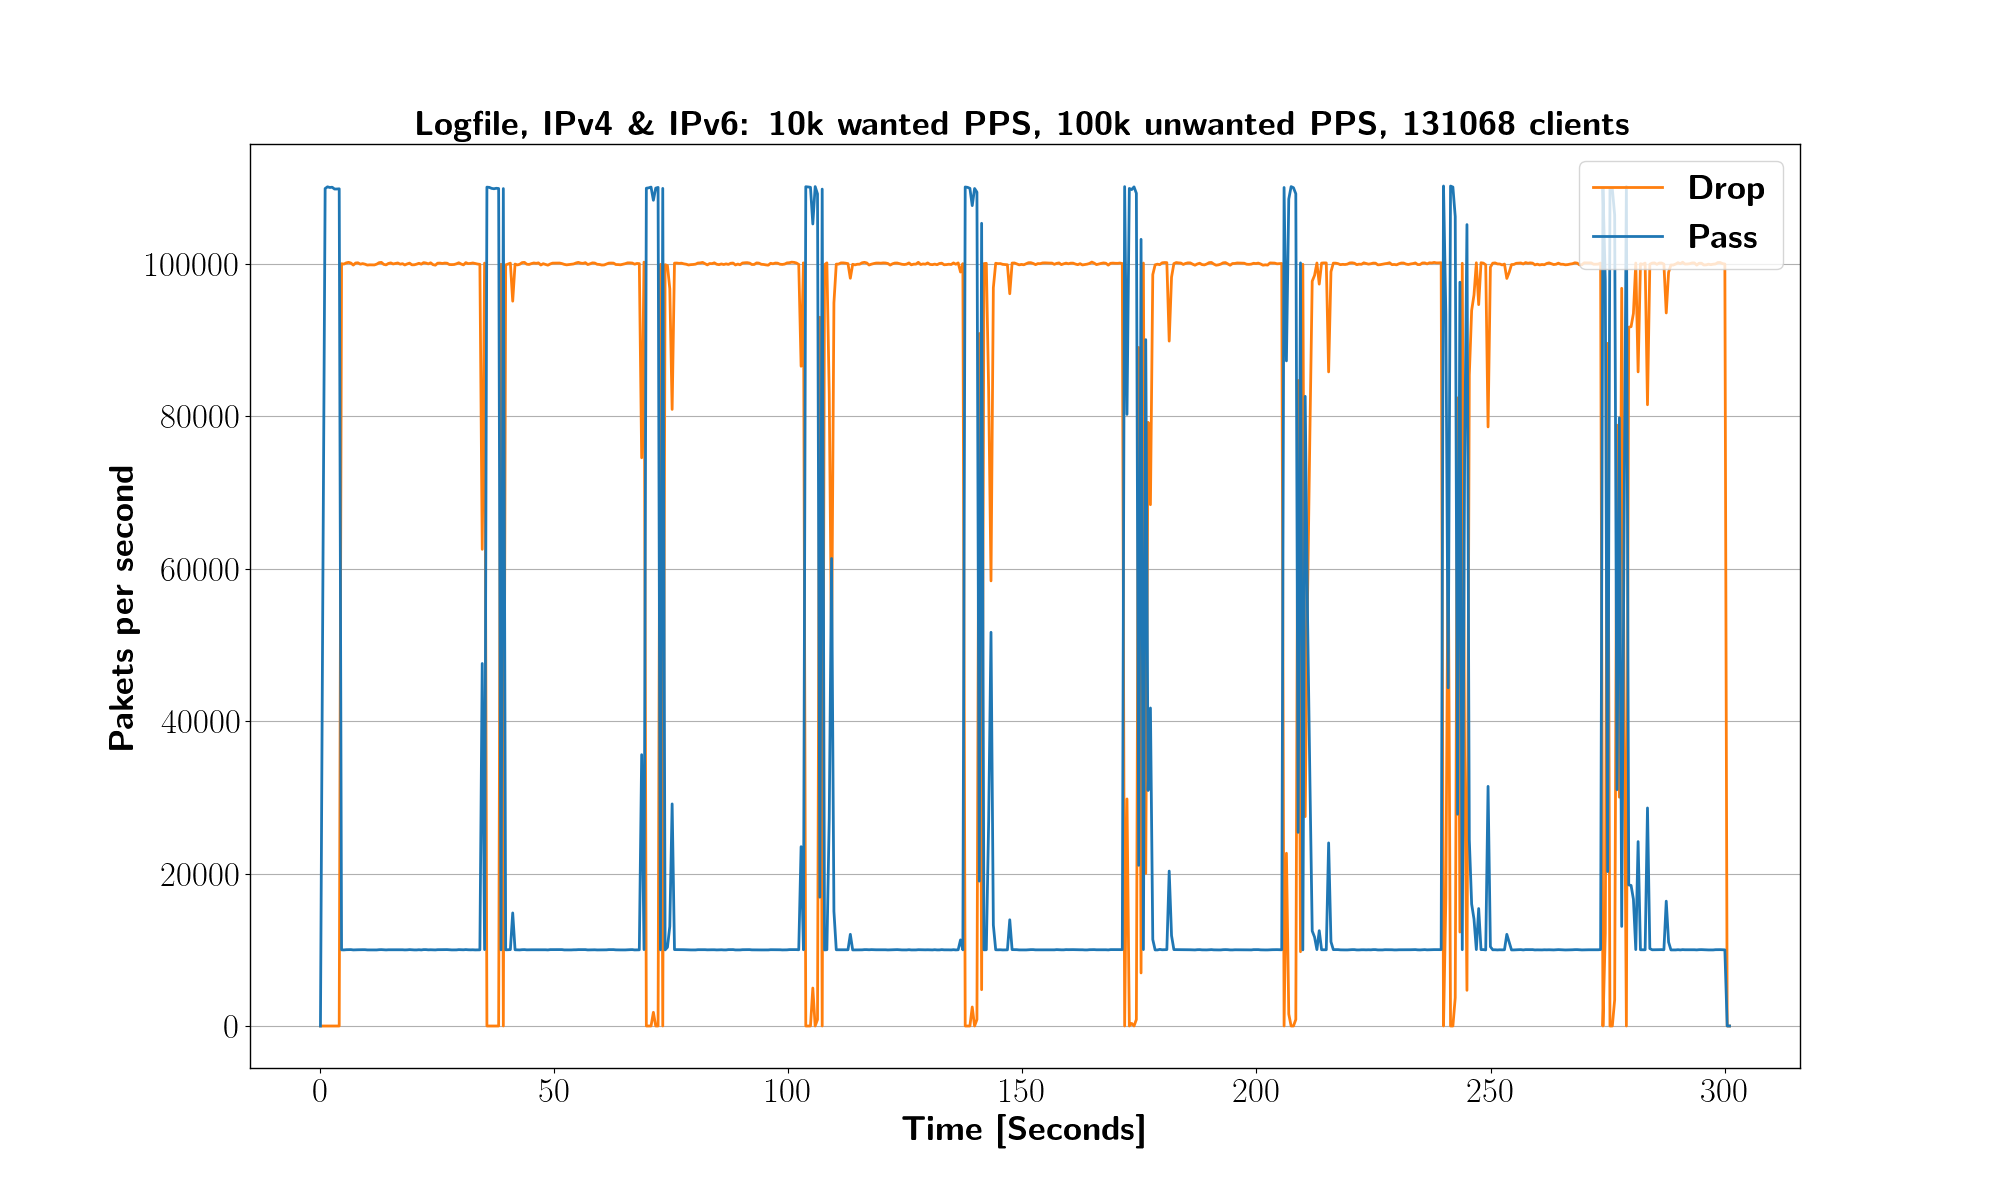
\includegraphics[width=1.2\textwidth]{images/simplefail2ban_disk_ipv46_v10k_iv100k_c131068.png}}
	\end{tabular}
	\begin{tabular}{lllll}
		\toprule
		\textbf{Total packets [$10^6$]} & \textbf{Packets dropped [$10^6$]} & \textbf{Relative drop [\%]} & \textbf{Log messages [$10^6$]} & \textbf{CPU [seconds]} \\ \midrule 
		33 & 26.45 & 99.96 & 3.55 & 18.47 \\
	\bottomrule
	\end{tabular}
	\caption[Simplefail2ban, Logfile IPv4 \& IPv6, 100k \ac{PPS}]{Some text}
	\label{fig:simplefail2ban:disk:ip46:100k}
\end{figure}

Figure \ref{fig:simplefail2ban:disk:ip46:100k} and figures \ref{fig:simplefail2ban:disk:ip4:100k}, \ref{fig:simplefail2ban:disk:ip6:100k} in the annex, present the results
for the logfile based Simplefail2ban at a traffic rate of 100 thousand invalid \ac{PPS}. Overall, the results are very similar for all three measurements and generally, over 99\% percentage of invalid traffic is dropped.
The visible gap between ban cycles can be explained by the test setup. TRex iterates over all clients address sequentially when sending traffic and the ban limit requires each client to at least
send at  least three packets before being banned. At a rate of 100k invalid request a second, this can take several seconds, dependant on the number of clients.
One slightly unexpected observation is, that the unbanning of clients does not always appear to occur at the same time, which increases for subsequent ban cycles.
A possible explanation for this is, that the timeout value for the unbanning thread was chosen to coarsely at 0.5 seconds. When the unbanning
thread iterates over the list of banned clients without performing a unbanning action, the thread will sleep for the specified timeout
before checking the list again. If poorly timed, this could lead to gaps between the unbanning of clients, which accumulate over time. Since the same
behavior is observed in later measurement, this issue should be investigated, if the development of Simplefail2ban is continued.   \\  

\begin{figure}[!h]
	\centering
	\scriptsize
	\begin{tabular}{c}
    	\centerline{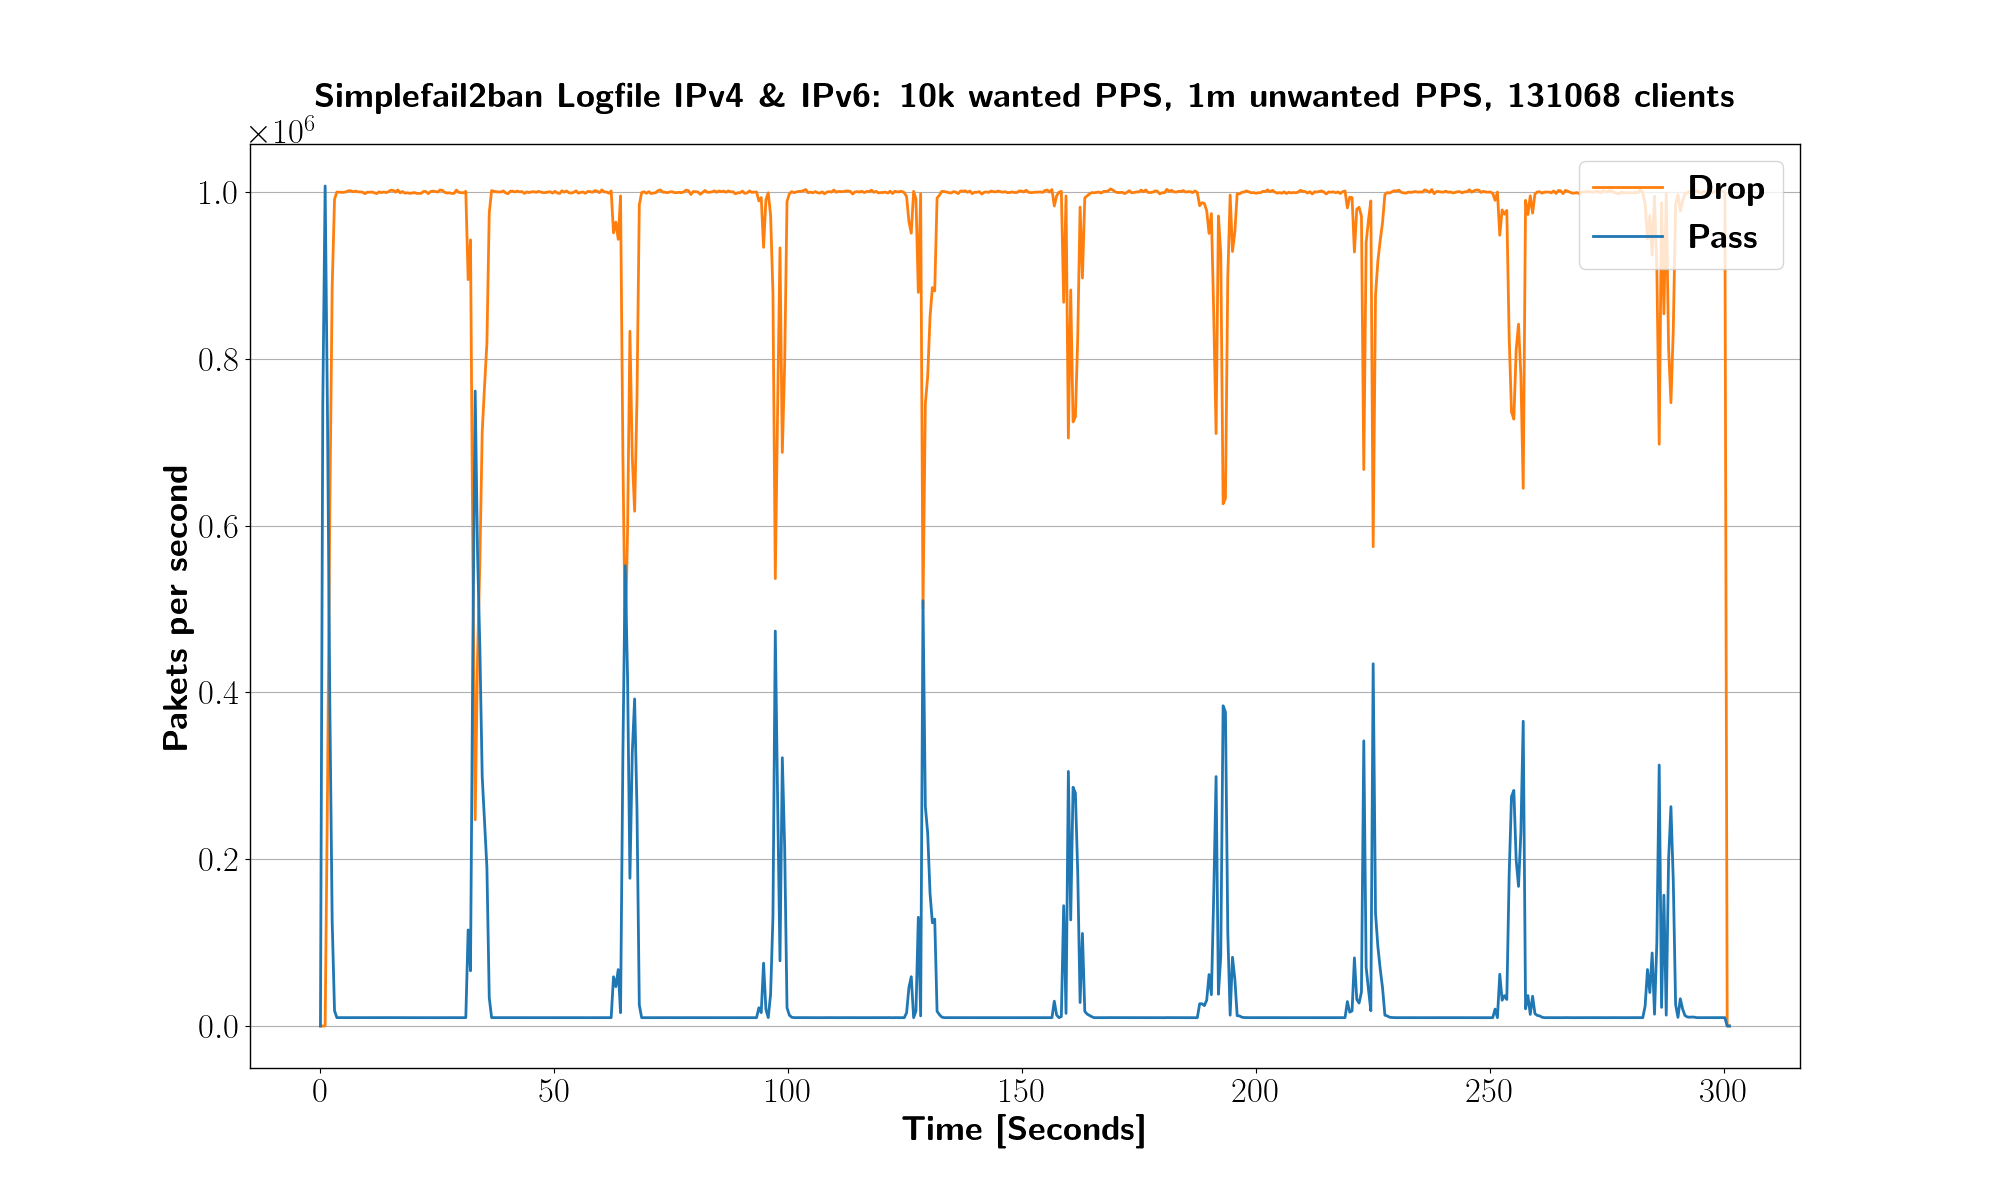
\includegraphics[width=1.2\textwidth]{images/simplefail2ban_disk_ipv46_v10k_iv1m_c131068.png}}
	\end{tabular}
	\begin{tabular}{lllll}
		\toprule
		\textbf{Total packets [$10^6$]} & \textbf{Packets dropped [$10^6$]} & \textbf{Relative drop [\%]} & \textbf{Log messages [$10^6$]} & \textbf{CPU [seconds]} \\ \midrule 
		303 & 290.47 & 98.11 & 8.5 & 32.94 \\
	\bottomrule
	\end{tabular}
	\caption[Simplefail2ban, Logfile IPv4 \& IPv6, 1m \ac{PPS}]{Some text}
	\label{fig:simplefail2ban:disk:ip46:1m}
\end{figure}

Figure \ref{fig:simplefail2ban:disk:ip46:1m} and figures \ref{fig:simplefail2ban:disk:ip4:1m}, \ref{fig:simplefail2ban:disk:ip6:1m} in the annex, present the results
for the logfile based Simplefail2ban at a traffic rate of 1 million invalid \ac{PPS}. Again, the result are very similar for all three measurement. Compared to the results at 100 thousand \ac{PPS},
the relative drops by about one percentage point across the measurements to around 98\%. The relative drop for the joint \ac{IPv4} \& \ac{IPv6} measurement is also slightly worse by about half a percentage point, than the
other two measurements, which can be explained by the fact, that the double the amount clients need to be banned and unbanned. The pure \ac{IPv4} measurement also slightly outperforms pure \ac{IPv6} in terms of relative
drop rate. This is likely the result of longer log messages due to the length of the \ac{IPv6}, which is more taxing for both the file reading as well as the \ac{Regex} matching.      

\begin{figure}[!h]
	\centering
	\scriptsize
	\begin{tabular}{c}
    	\centerline{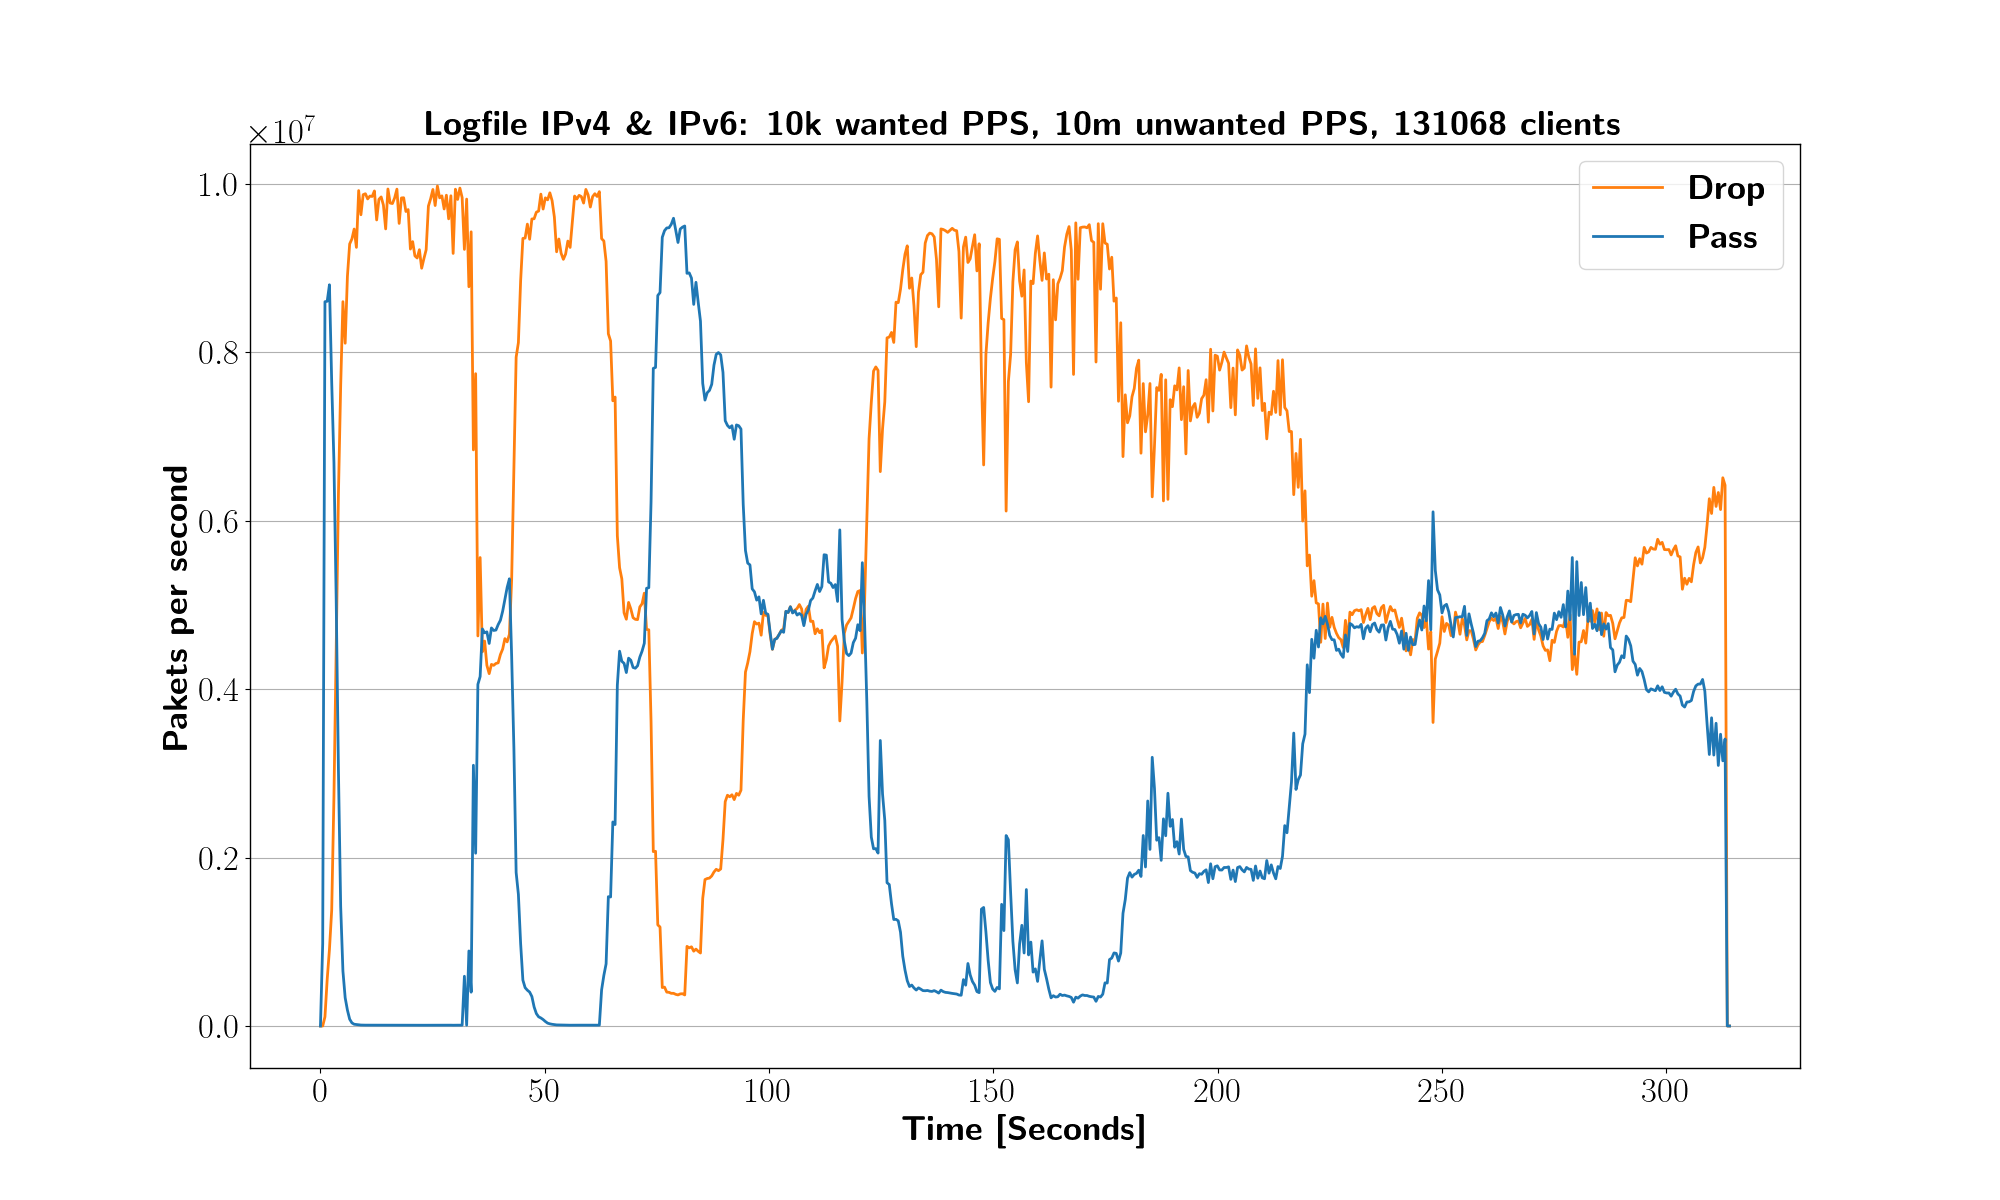
\includegraphics[width=1.2\textwidth]{images/simplefail2ban_disk_ipv46_v10k_iv10m_c131068.png}}
	\end{tabular}
	\begin{tabular}{lllll}
		\toprule
		\textbf{Total packets [$10^6$]} & \textbf{Packets dropped [$10^6$]} & \textbf{Relative drop [\%]} & \textbf{Log messages [$10^6$]} & \textbf{CPU [seconds]} \\ \midrule 
		2993.57 & 2014.77 & 67.46 & 213.63 & 382.19 \\
		\bottomrule
	\end{tabular}
	\caption[Simplefail2ban, Logfile IPv4 \& IPv6, 10m \ac{PPS}]{Some text}
	\label{fig:simplefail2ban:disk:ip46:10m}
\end{figure}

Finally, figure \ref{fig:simplefail2ban:disk:ip46:10m} and figures \ref{fig:simplefail2ban:disk:ip4:10m}, \ref{fig:simplefail2ban:disk:ip6:10m} in the annex, present the results
for the logfile based Simplefail2ban at a traffic rate of 10 million invalid \ac{PPS}. Compared to the previous result, overall performance drops drastically. The best result is achieved for the purpose
\ac{IPv4} traffic, which maintains a high relative drop rate of 96.72 \%, even though CPU usage and the amount of messages processes are about 6 times 
higher than in 1 million \ac{PPS} measurement. For \ac{IPv6} and the joint traffic, result are much worse, as only around 69\% and 67\% of the expected traffic is dropped.
The results are similar to those of Fail2ban in figure \ref{fig:fail2ban:mikolajczak2022}. Simplefail2ban appears to be overwhelmed with the processing of log messages at a certain point and
does not manage to recover before the end of the ban cycle. For the \ac{IPv6} measurement Simplefail2ban managed to process only about 89\% of the total log messages written by the server. For the joint measurement
the number is significantly lower at around 64\%. Overall the result show, that, even though the threshold appears to be larger, the same issues of file based log message parsing persist for Simplefail2ban.

\pagebreak

\subsection{Experiment 3: Shared Memory Variant}


\begin{figure}[!h]
	\label{fig:simplefail2ban:shm:ip46:100k}
	\centering
	\scriptsize
	\begin{tabular}{c}
    	\centerline{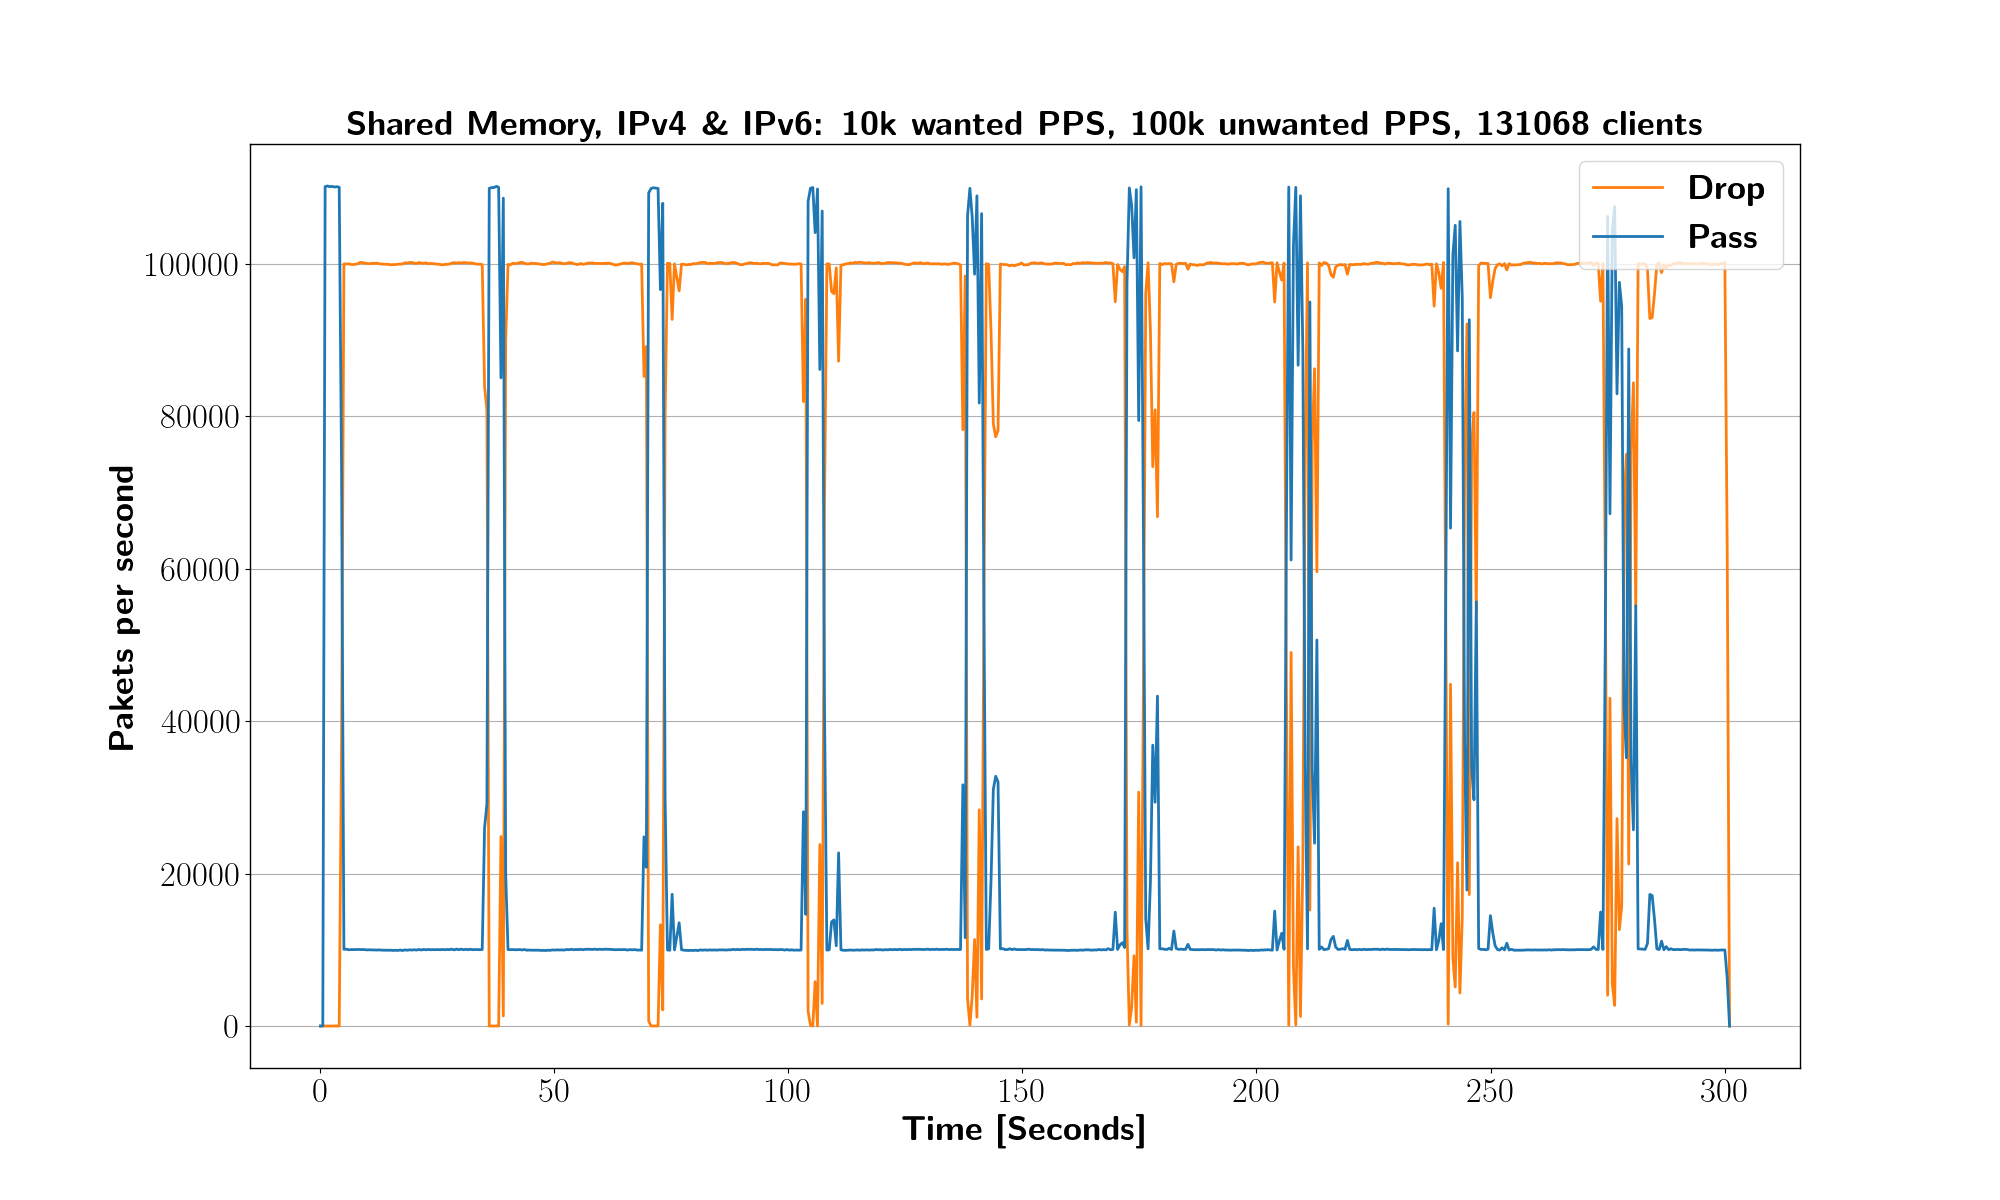
\includegraphics[width=1.2\textwidth]{images/simplefail2ban_shm_ipv46_v10k_iv100k_c131068.png}}
	\end{tabular}
	\begin{tabular}{lllll}
		\toprule
		\textbf{Total packets [$10^6$]} & \textbf{Packets dropped [$10^6$]} & \textbf{Relative drop [\%]} & \textbf{Log messages [$10^6$]} & \textbf{CPU [seconds]} \\ \midrule 
		33 & 26.45 & 99.95 & 3.55 & 26.35 \\
		\bottomrule
	\end{tabular}
	\caption[Simplefail2ban, Shared Memory, IPv4 \& IPv6, 100k \ac{PPS}]{Some text}
\end{figure}

Figure \ref{fig:simplefail2ban:shm:ip46:100k} and figures \ref{fig:simplefail2ban:shm:ip4:100k}, \ref{fig:simplefail2ban:shm:ip6:100k} in the annex, present the results
for the logfile based Simplefail2ban at a traffic rate of 100 thousand invalid \ac{PPS}. All three measurements show similar results, which are also similar two the result measured for the logfile-based
version of Simplefail2ban. Again a relative drop rate of over 99\% percent is achieved across the board. The only noticeable difference to logfile-based result is, that the \ac{CPU} usage appear to be slightly higher.
However, this observation is skewed by the fact, that the execution time of the kernel performing the io\_uring based reads is not included in the statistic. 

\pagebreak

\begin{figure}[!h]
	\label{fig:simplefail2ban:shm:ip46:1m}
	\centering
	\scriptsize
	\begin{tabular}{c}
    	\centerline{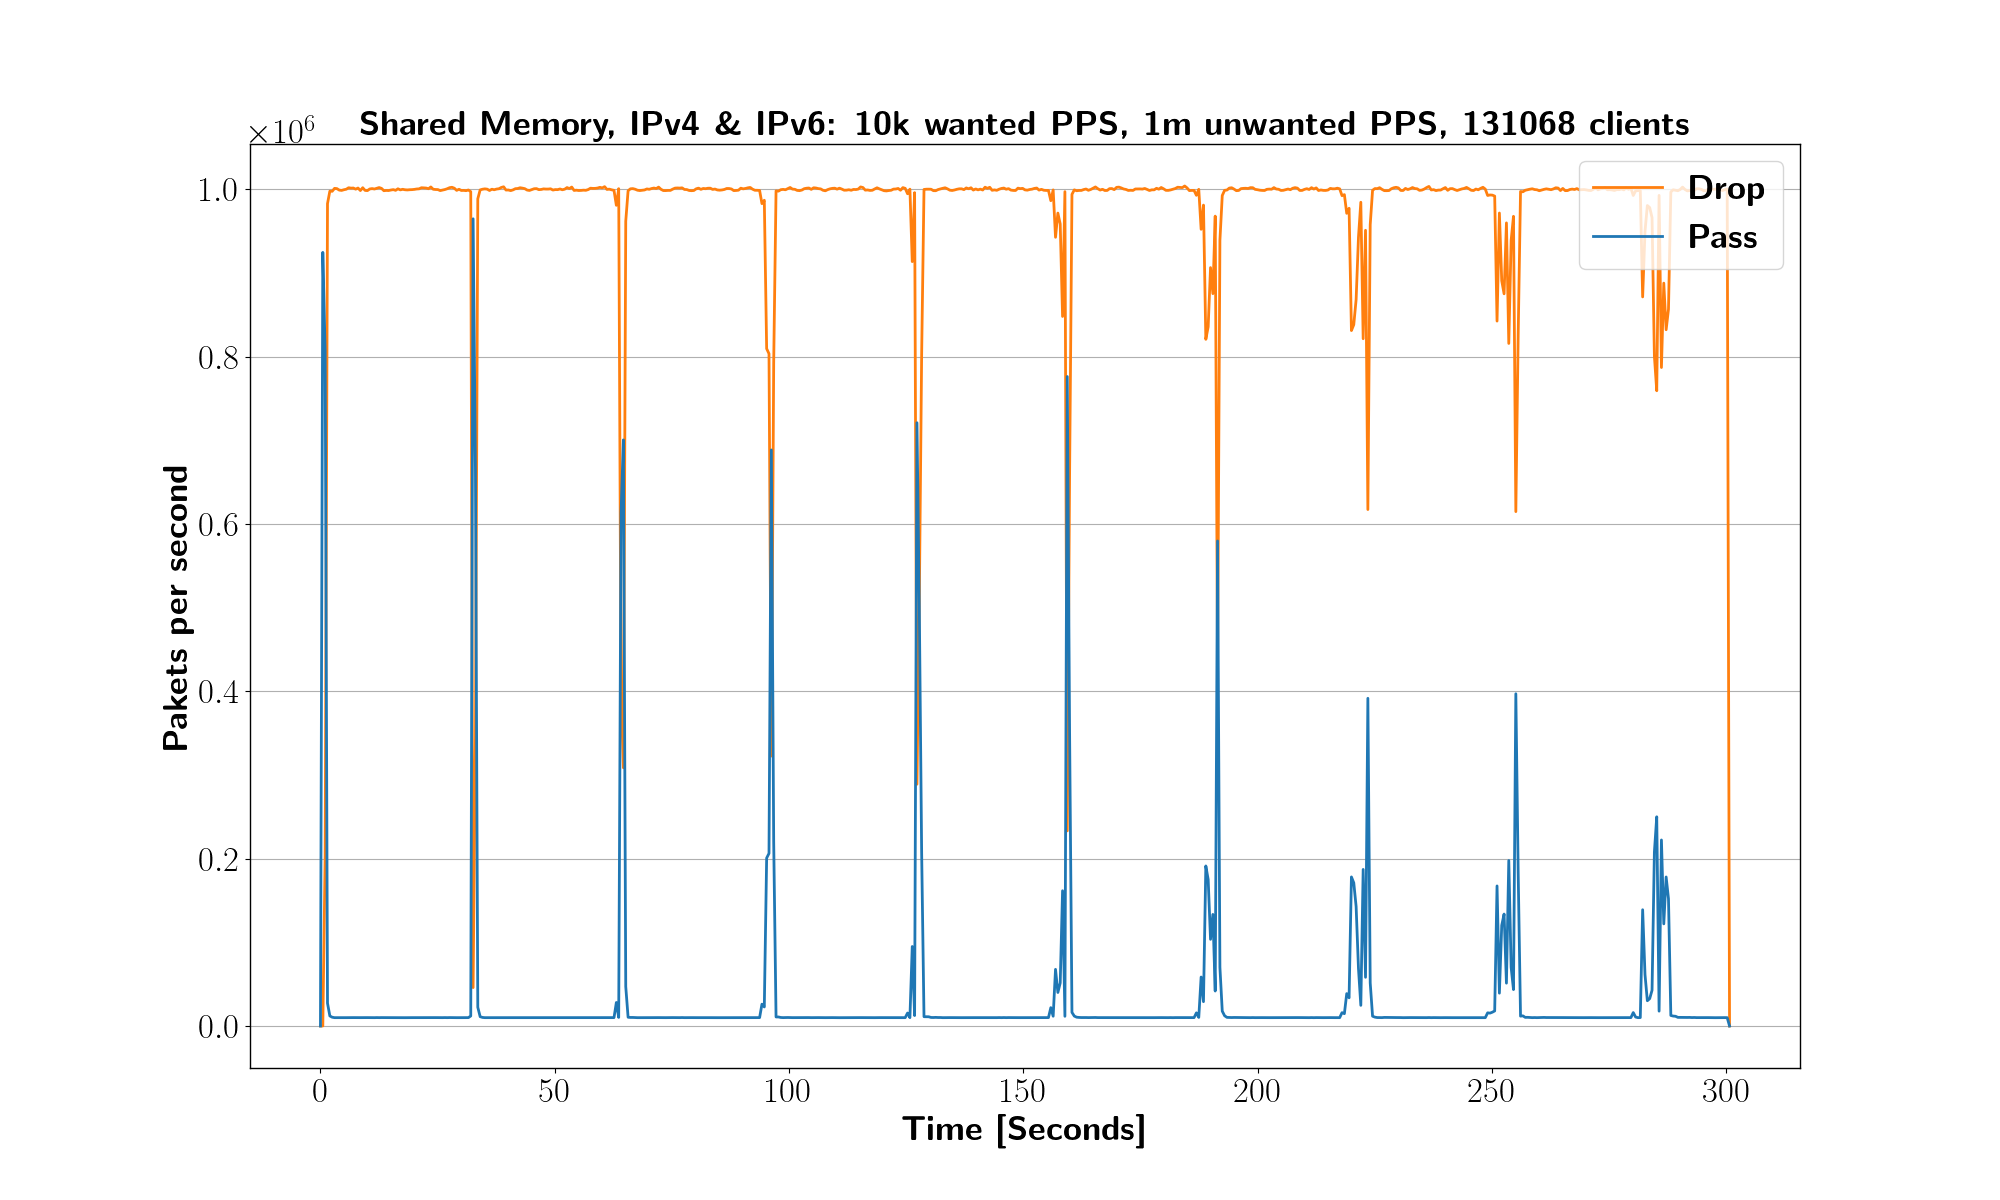
\includegraphics[width=1.2\textwidth]{images/simplefail2ban_shm_ipv46_v10k_iv1m_c131068.png}}
	\end{tabular}
	\begin{tabular}{lllll}
		\toprule
		\textbf{Total packets [$10^6$]} & \textbf{Packets dropped [$10^6$]} & \textbf{Relative drop [\%]} & \textbf{Log messages [$10^6$]} & \textbf{CPU [seconds]} \\ \midrule 
		303 & 293.13 & 99 & 5.95 & 27.66 \\
		\bottomrule
	\end{tabular}
	\caption[Simplefail2ban, Shared Memory, IPv4 \& IPv6, 1m \ac{PPS}]{Some text}
\end{figure}

Figure \ref{fig:simplefail2ban:shm:ip46:1m} and figures \ref{fig:simplefail2ban:shm:ip4:1m}, \ref{fig:simplefail2ban:shm:ip6:1m} in the annex, present the results
for the logfile based Simplefail2ban at a traffic rate of 1 million invalid \ac{PPS}. Again, the results are very similar, both between the measurements, as well as compared to the logfile-based
measurements. Overall, the shared memory based Fail2ban performs slightly better across the board, with a relative drop rate of around 99\%. Interestingly, there appears 
to be no significant performance difference between the pure \ac{IPv4} and \ac{IPv6} and the joint measurements, even though
the latter has to process double the amount of clients.

\pagebreak

\begin{figure}[!h]
	\label{fig:simplefail2ban:shm:ip46:10m}
	\centering
	\scriptsize
	\begin{tabular}{c}
    	\centerline{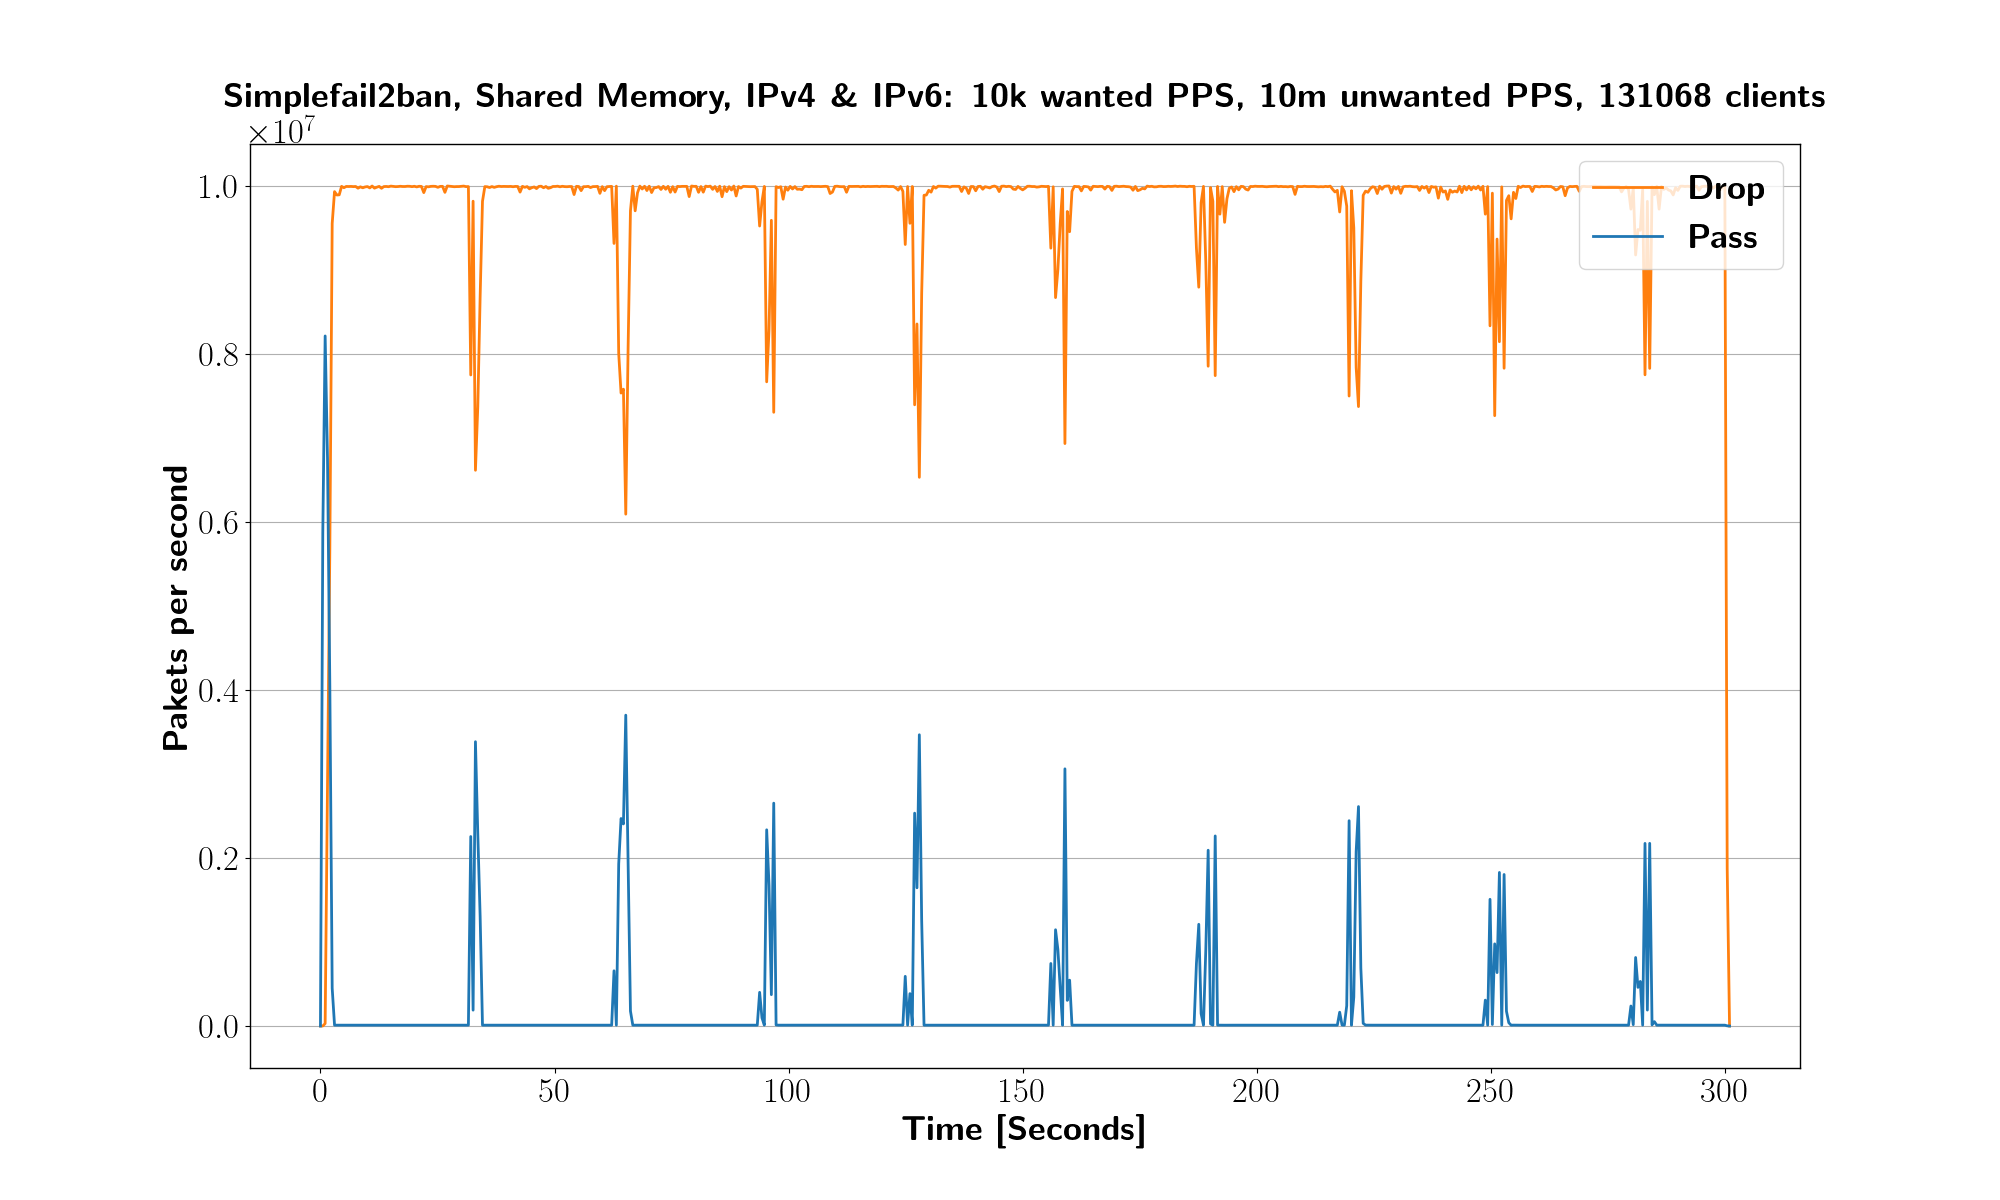
\includegraphics[width=1.2\textwidth]{images/simplefail2ban_shm_ipv46_v10k_iv10m_c131068.png}}
	\end{tabular}
	\begin{tabular}{lllll}
		\toprule
		\textbf{Total packets [$10^6$]} & \textbf{Packets dropped [$10^6$]} & \textbf{Relative drop [\%]} & \textbf{Log messages [$10^6$]} & \textbf{CPU [seconds]} \\ \midrule 
		2992.44 & 2939.27 & 98.45 & 16.18 & 65.74 \\
		\bottomrule
	\end{tabular}
	\caption[Simplefail2ban, Shared Memory, IPv4 \& IPv6, 10m \ac{PPS}]{Some text}
\end{figure}

Figure \ref{fig:simplefail2ban:shm:ip46:10m} and figures \ref{fig:simplefail2ban:shm:ip4:10m}, \ref{fig:simplefail2ban:shm:ip6:10m} in the annex, present the results
for the logfile based Simplefail2ban at a traffic rate of 10 million invalid \ac{PPS}. Compared to the previous logfile-based measurements,
performance is a lot better. Both the \ac{IPv6} and joint measurements achieved a relative drop rate of more than 98\%. Counterintuitively, the
pure \ac{IPv4} measurement performed the worst, at only 96.72 \%. The reason for this is not entirely clear, but it may be further
indication that the performance of Simplefail2ban varies more than the initial measurements indicated. Hence, further replication
is necessary to provide a more stable estimation of the expected performance. 

\pagebreak

\begin{figure}[!h]
	\centering
	\scriptsize
	\begin{tabular}{c}
    	\centerline{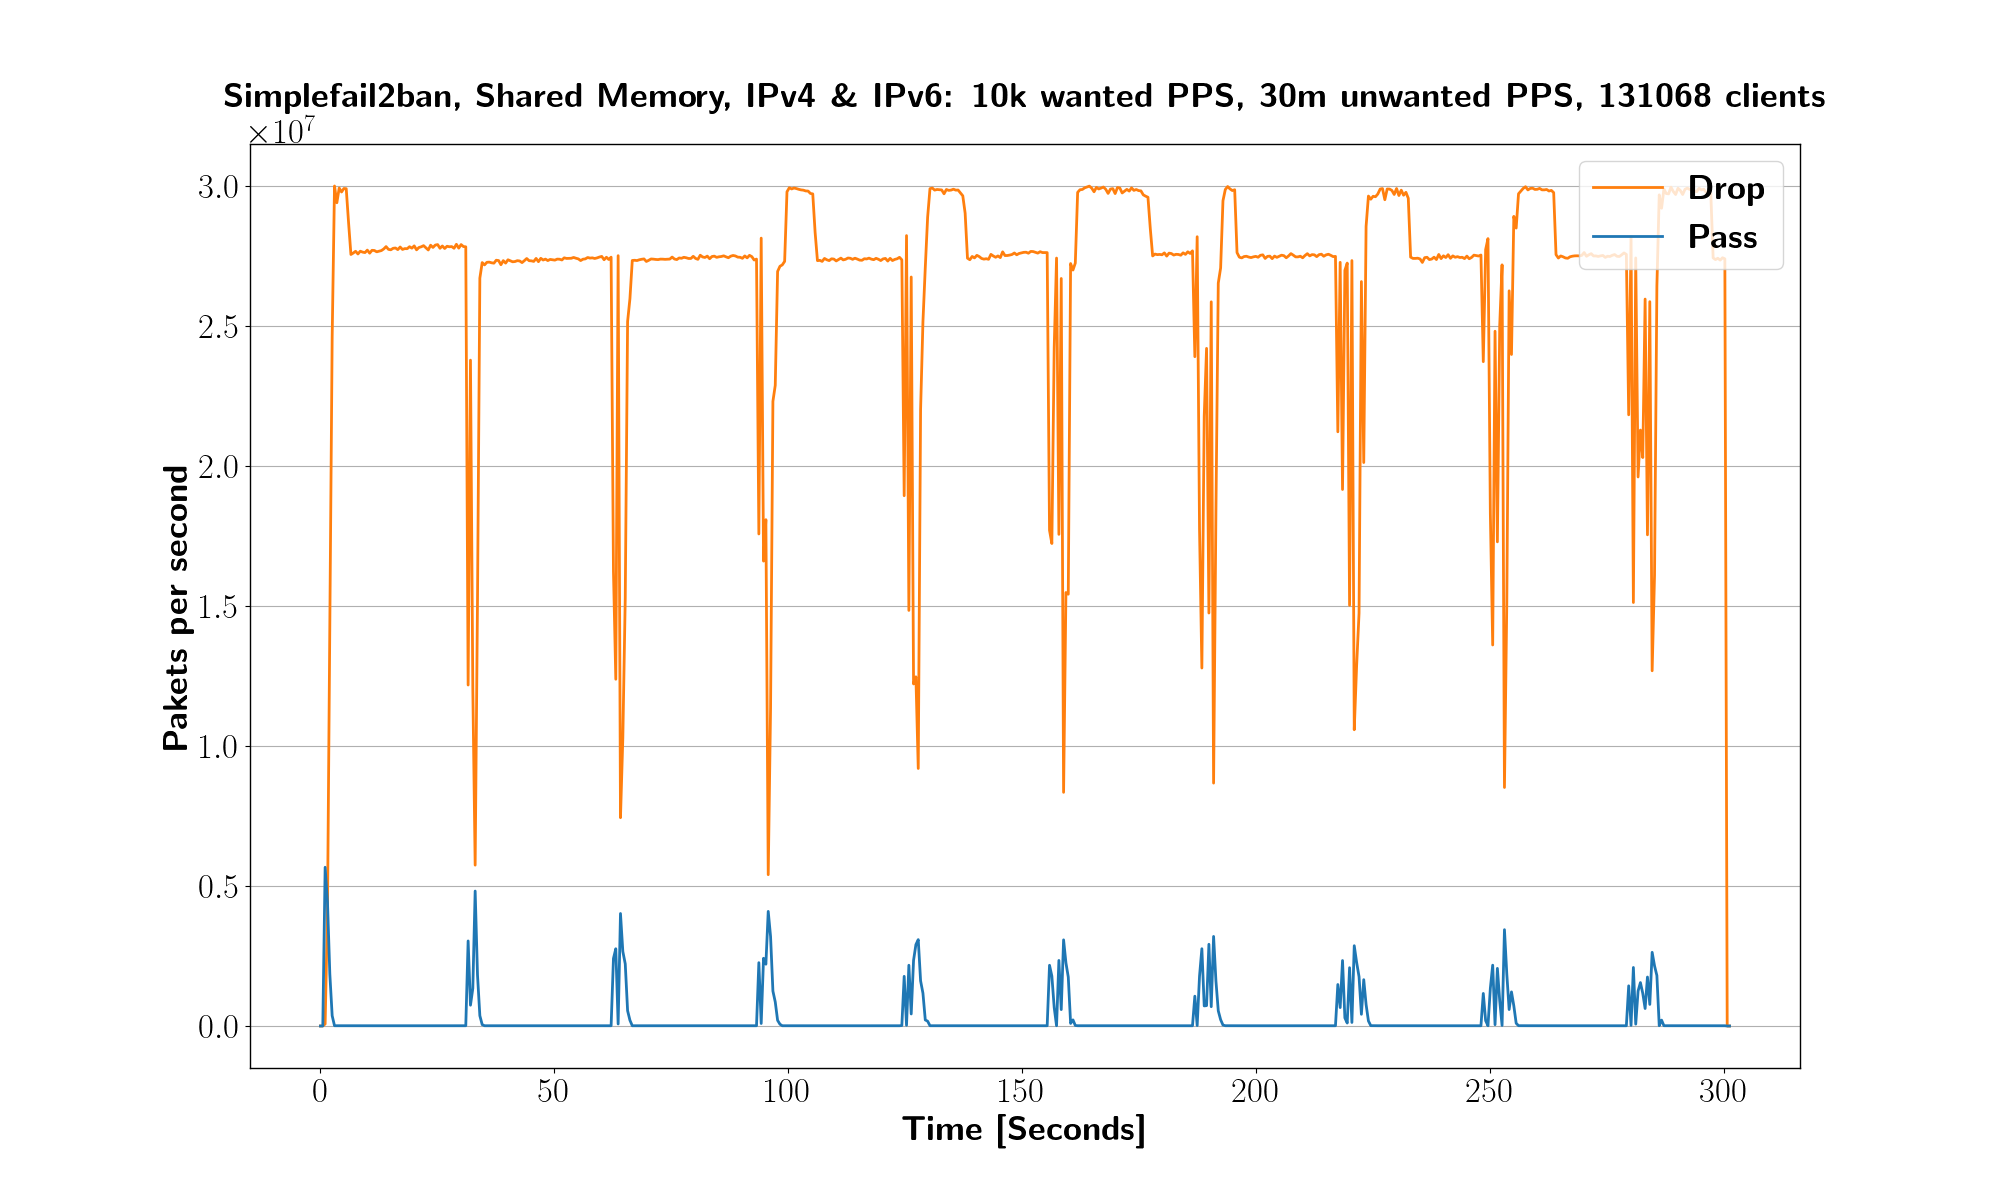
\includegraphics[width=1.2\textwidth]{images/simplefail2ban_shm_ipv46_v10k_iv30m_c131068.png}}
	\end{tabular}
	\begin{tabular}{lllll}
		\toprule
		\textbf{Total packets [$10^6$]} & \textbf{Packets dropped [$10^6$]} & \textbf{Relative drop [\%]} & \textbf{Log messages [$10^6$]} & \textbf{CPU [seconds]} \\ \midrule 
		8095.28 & 8017.72 & 99.13 & 21 & 76.23 \\
		\bottomrule
	\end{tabular}
	\caption[Simplefail2ban, Shared Memory, IPv4 \& IPv6, 30m \ac{PPS}]{Some text}
	\label{fig:simplefail2ban:shm:ip46:30m}
\end{figure}

Finally, figure \ref{fig:simplefail2ban:shm:ip46:30m} presents the results for a supplementary measurement of the 
shared memory based Simplefail2ban. For this measurements, the invalid traffic rate was increased to 30 million \ac{PPS} in order to test the boundaries of the system in terms of traffic.  
Overall, performance was surprisingly good, since over 99\% of invalid traffic was successfully dropped. However, the results are likely skewed, as the system was not able handle
the entire incoming traffic. As evident by the variance in the drop curve, without corresponding increases in the number of passes packets, not all packets where parsed by the \ac{eBPF} program.
In total, only around 8.095 billion  packets out of 9.003 billion packets were registered. Similar behavior was already observed by Florian Mikolajczak \cite{mikolajczak2022} for traffic rates beyond
30 million packets per second.

\pagebreak

\subsection{Experiment 4: Shared Memory Features}

In the following, features of the shared memory implementation are evaluated. All measurements are conducted with same traffic and client levels as the measurements presented in figure \ref{fig:simplefail2ban:shm:ip46:10m}.
Hence, the measurement servers as a baseline for comparing performance difference with additionally enabled features.

\begin{figure}[!h]
	\centering
	\scriptsize
	\begin{tabular}{c}
    	\centerline{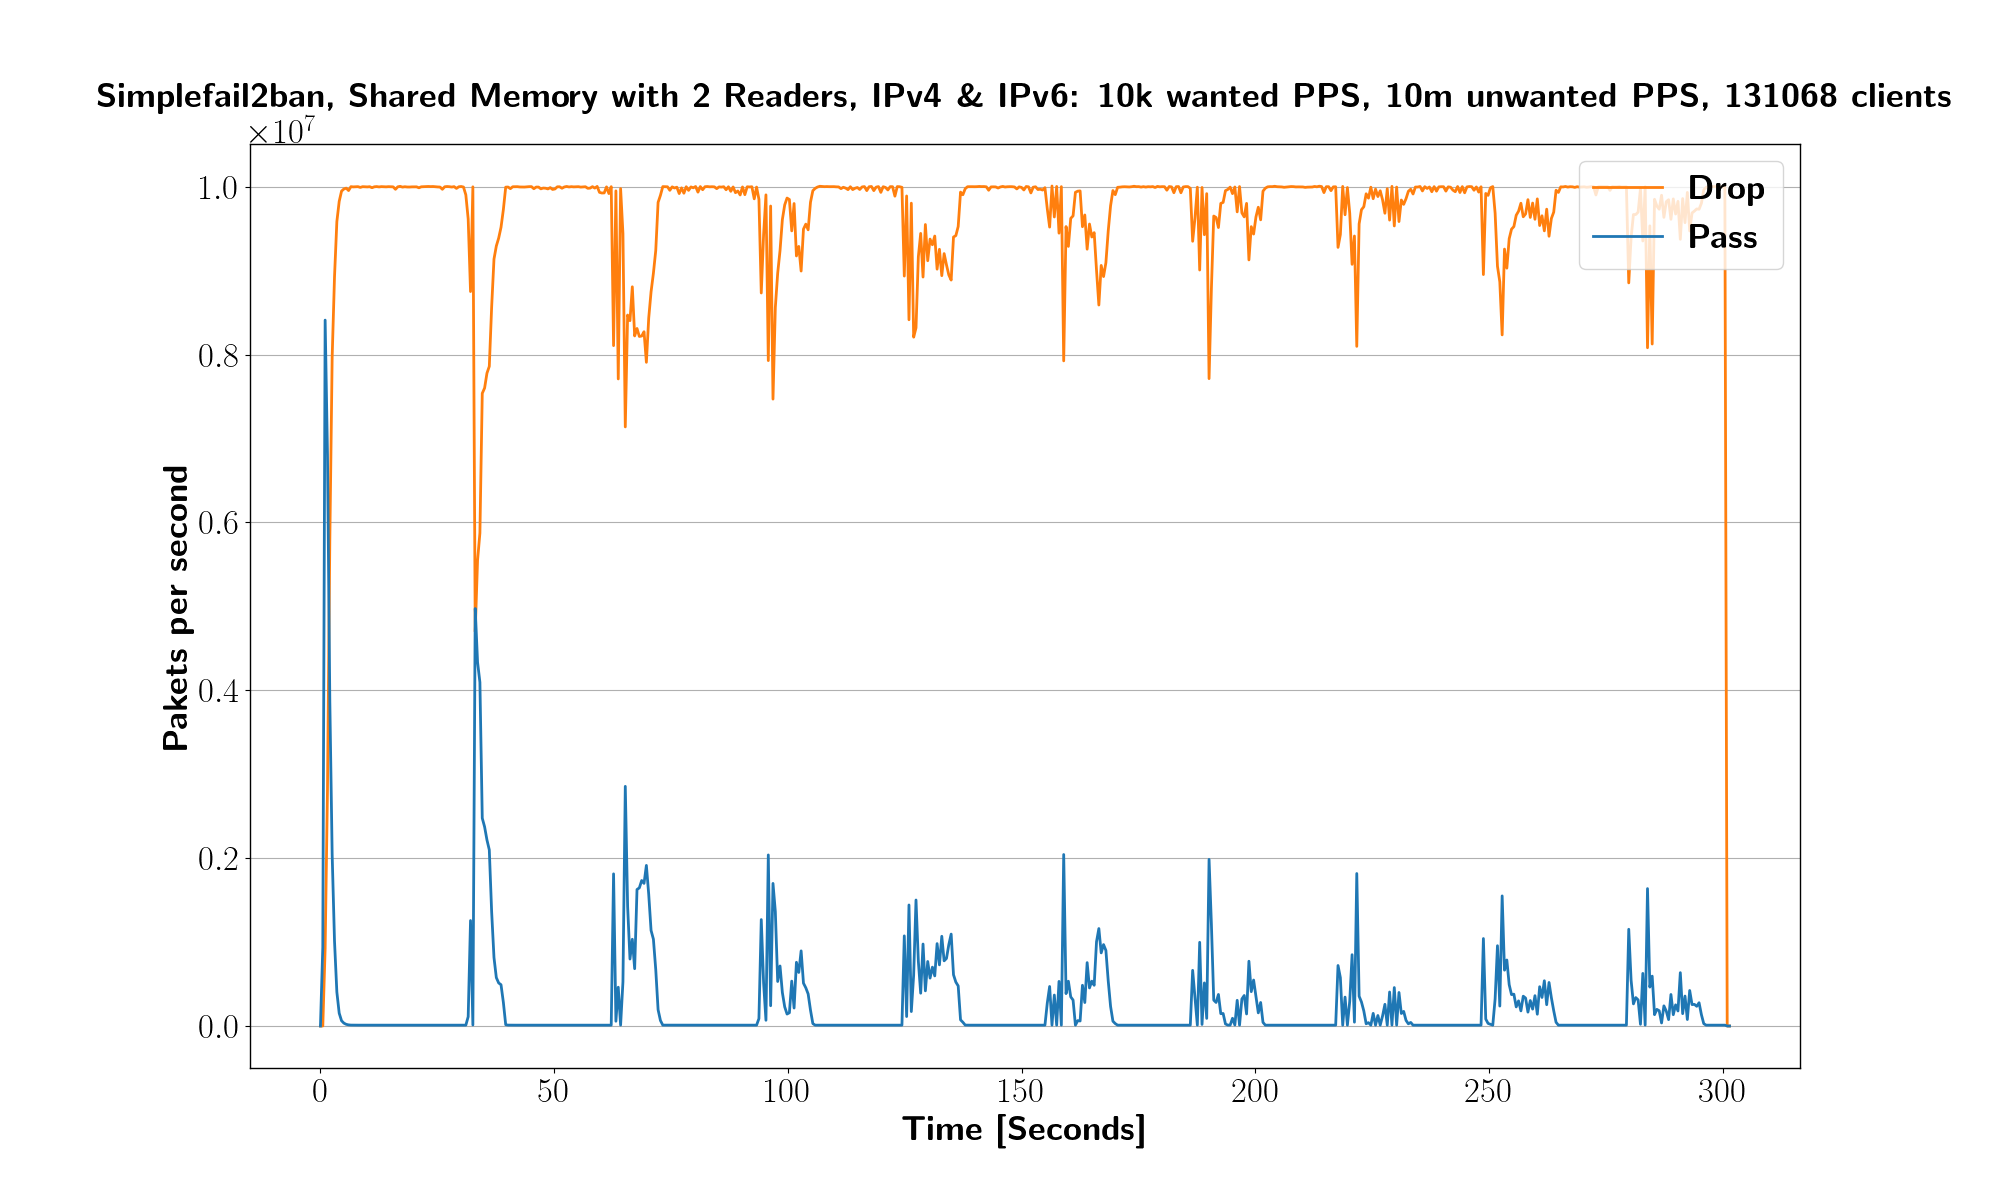
\includegraphics[width=1.2\textwidth]{images/simplefail2ban_shm_2r_ipv46_v10k_iv10m_c131068.png}}
	\end{tabular}
	\begin{tabular}{lllll}
		\toprule
		\textbf{Total packets [$10^6$]} & \textbf{Packets dropped [$10^6$]} & \textbf{Relative drop [\%]} & \textbf{Log messages [$10^6$]} & \textbf{CPU [seconds]} \\ \midrule 
		2989.66 & 2906.36 & 97.44 & 17.67 & 77.19 \\
		\bottomrule
	\end{tabular}
	\caption[Simplefail2ban, Shared Memory 2 Readers]{Some text}
	\label{fig:simplefail2ban:shm:2r}
\end{figure}

Figure \ref{fig:simplefail2ban:shm:2r} presents the results for shared memory Simplefail2ban with an additional reader attached to the buffer. For this purpose, the simplelogstash
program introduced in \ref{sec:other} was attached as a second reader, writing the contents of the buffer to a logfile. Compared to the baseline measurement, performance drops by about one percentage
point to 97.4\% of dropped invalid traffic. Additionally, the variance of when client are unbanned is noticeably larger
than in most of the previous measurements. This may caused by the fact, that the test server has to drop messages, as buffer reaches capacity due to the slower second reader.
About 54\% of all log messages by the server are dropped.   

\pagebreak

\begin{figure}[!h]
	\centering
	\scriptsize
	\begin{tabular}{c}
    	\centerline{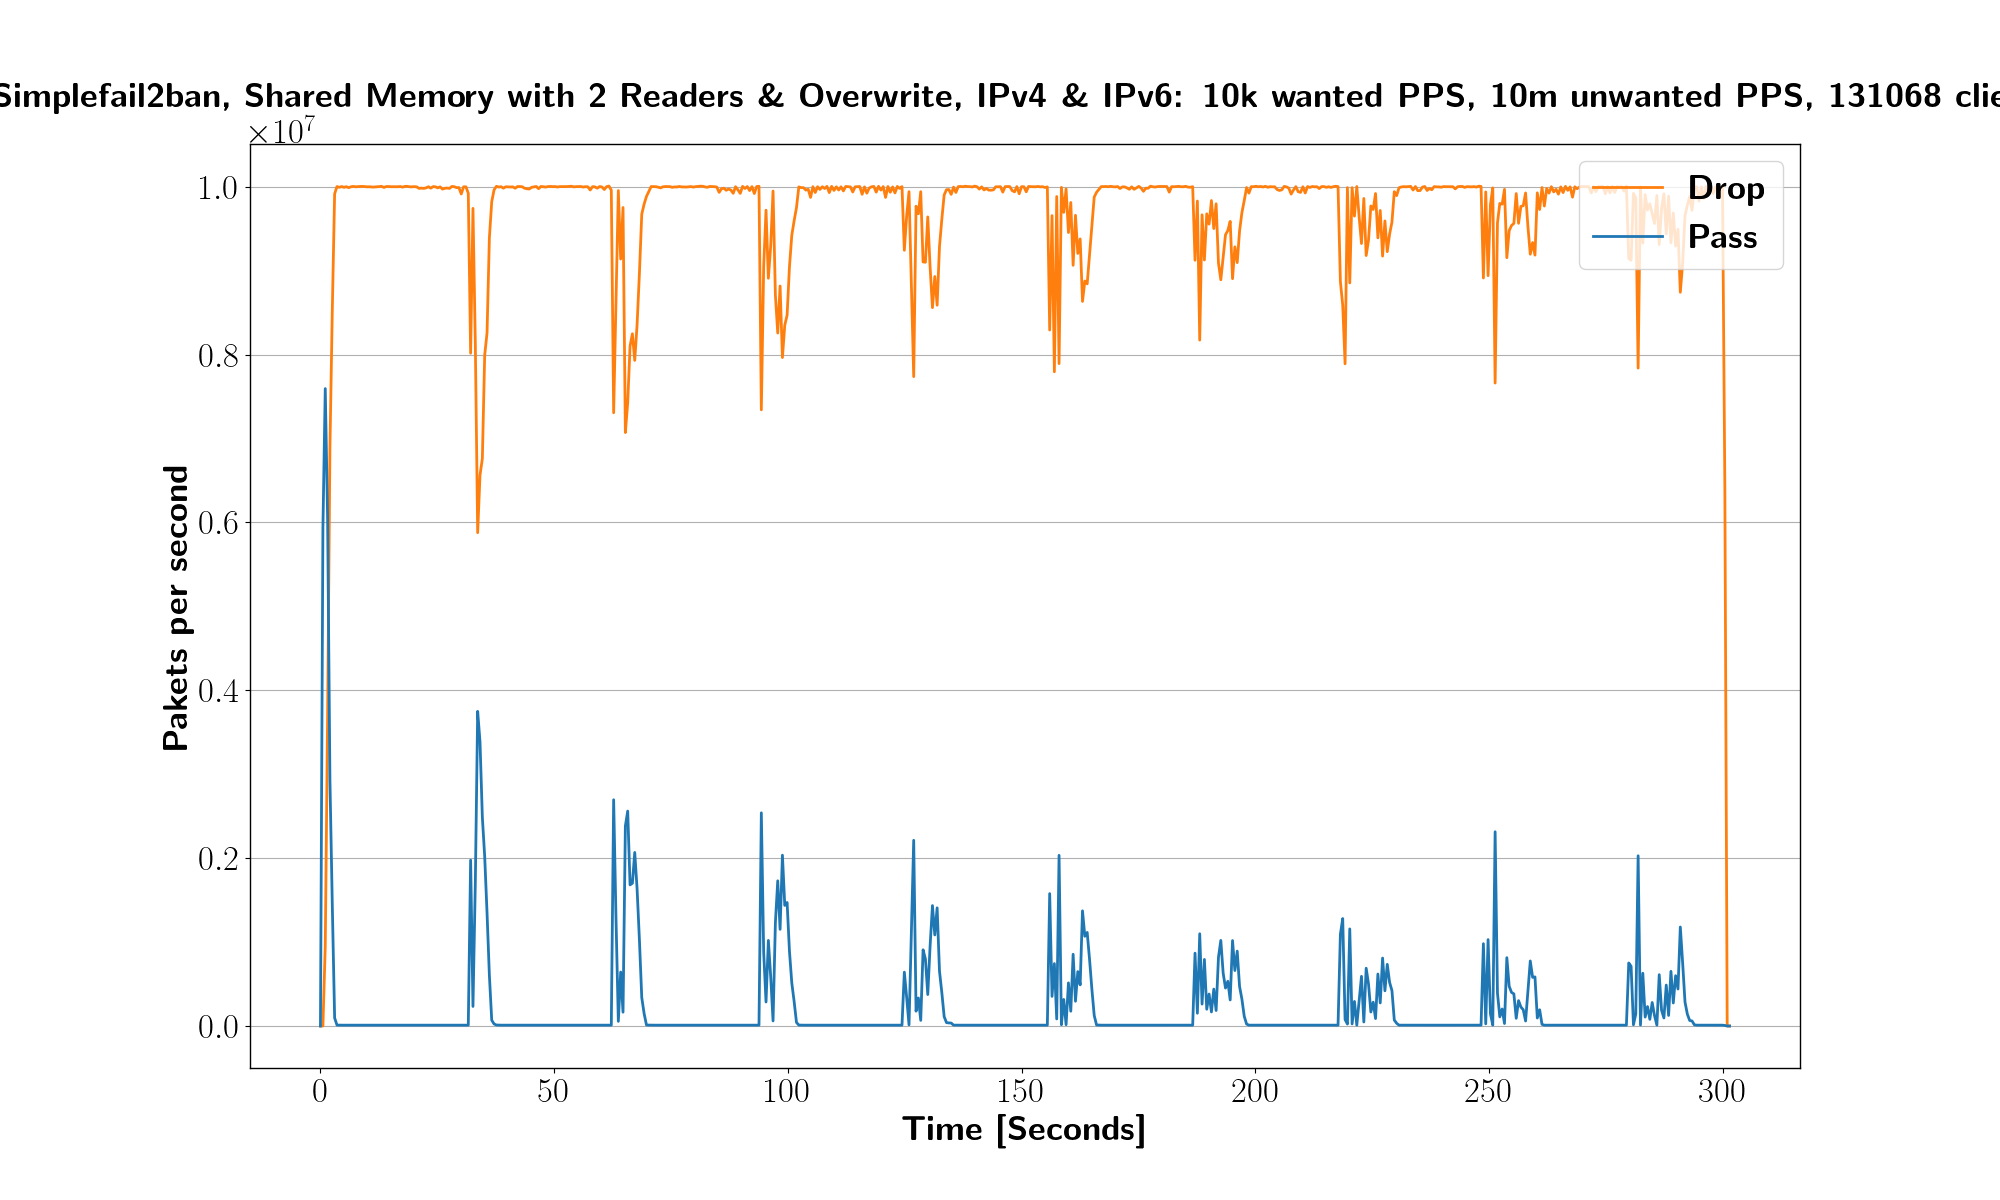
\includegraphics[width=1.2\textwidth]{images/simplefail2ban_shm_2r_or_ipv46_v10k_iv10m_c131068.png}}
	\end{tabular}
	\begin{tabular}{lllll}
		\toprule
		\textbf{Total packets [$10^6$]} & \textbf{Packets dropped [$10^6$]} & \textbf{Relative drop [\%]} & \textbf{Log messages [$10^6$]} & \textbf{CPU [seconds]} \\ \midrule 
		2988.9 & 2914.39 & 97.73 & 17.66 & 79.13 \\
		\bottomrule
	\end{tabular}
	\caption[Simplefail2ban, Shared Memory 2 Readers with Overwrite]{Some text}
	\label{fig:simplefail2ban:shm:or}
\end{figure}

Figure \ref{fig:simplefail2ban:shm:2r} presents the results for the two reader scenario with the additionally enabled overwrite feature. Contrary to expectation,
the performance is not significantly better, at less then a percentage point of dropped invalid traffic. Simplefail2ban only managed to read about 58\% of all log messages 
written by the server, while the second reader read only about 41\% of all messages. This behavior is unexpected and points at a potential bug in the implementation of the overwrite
feature. For potential further development of Simplefail2ban, the overwrite feature should be inspected closely and potentially revised, if performance does not improve. 

\pagebreak

\begin{figure}[!h]
	\centering
	\scriptsize
	\begin{tabular}{c}
    	\centerline{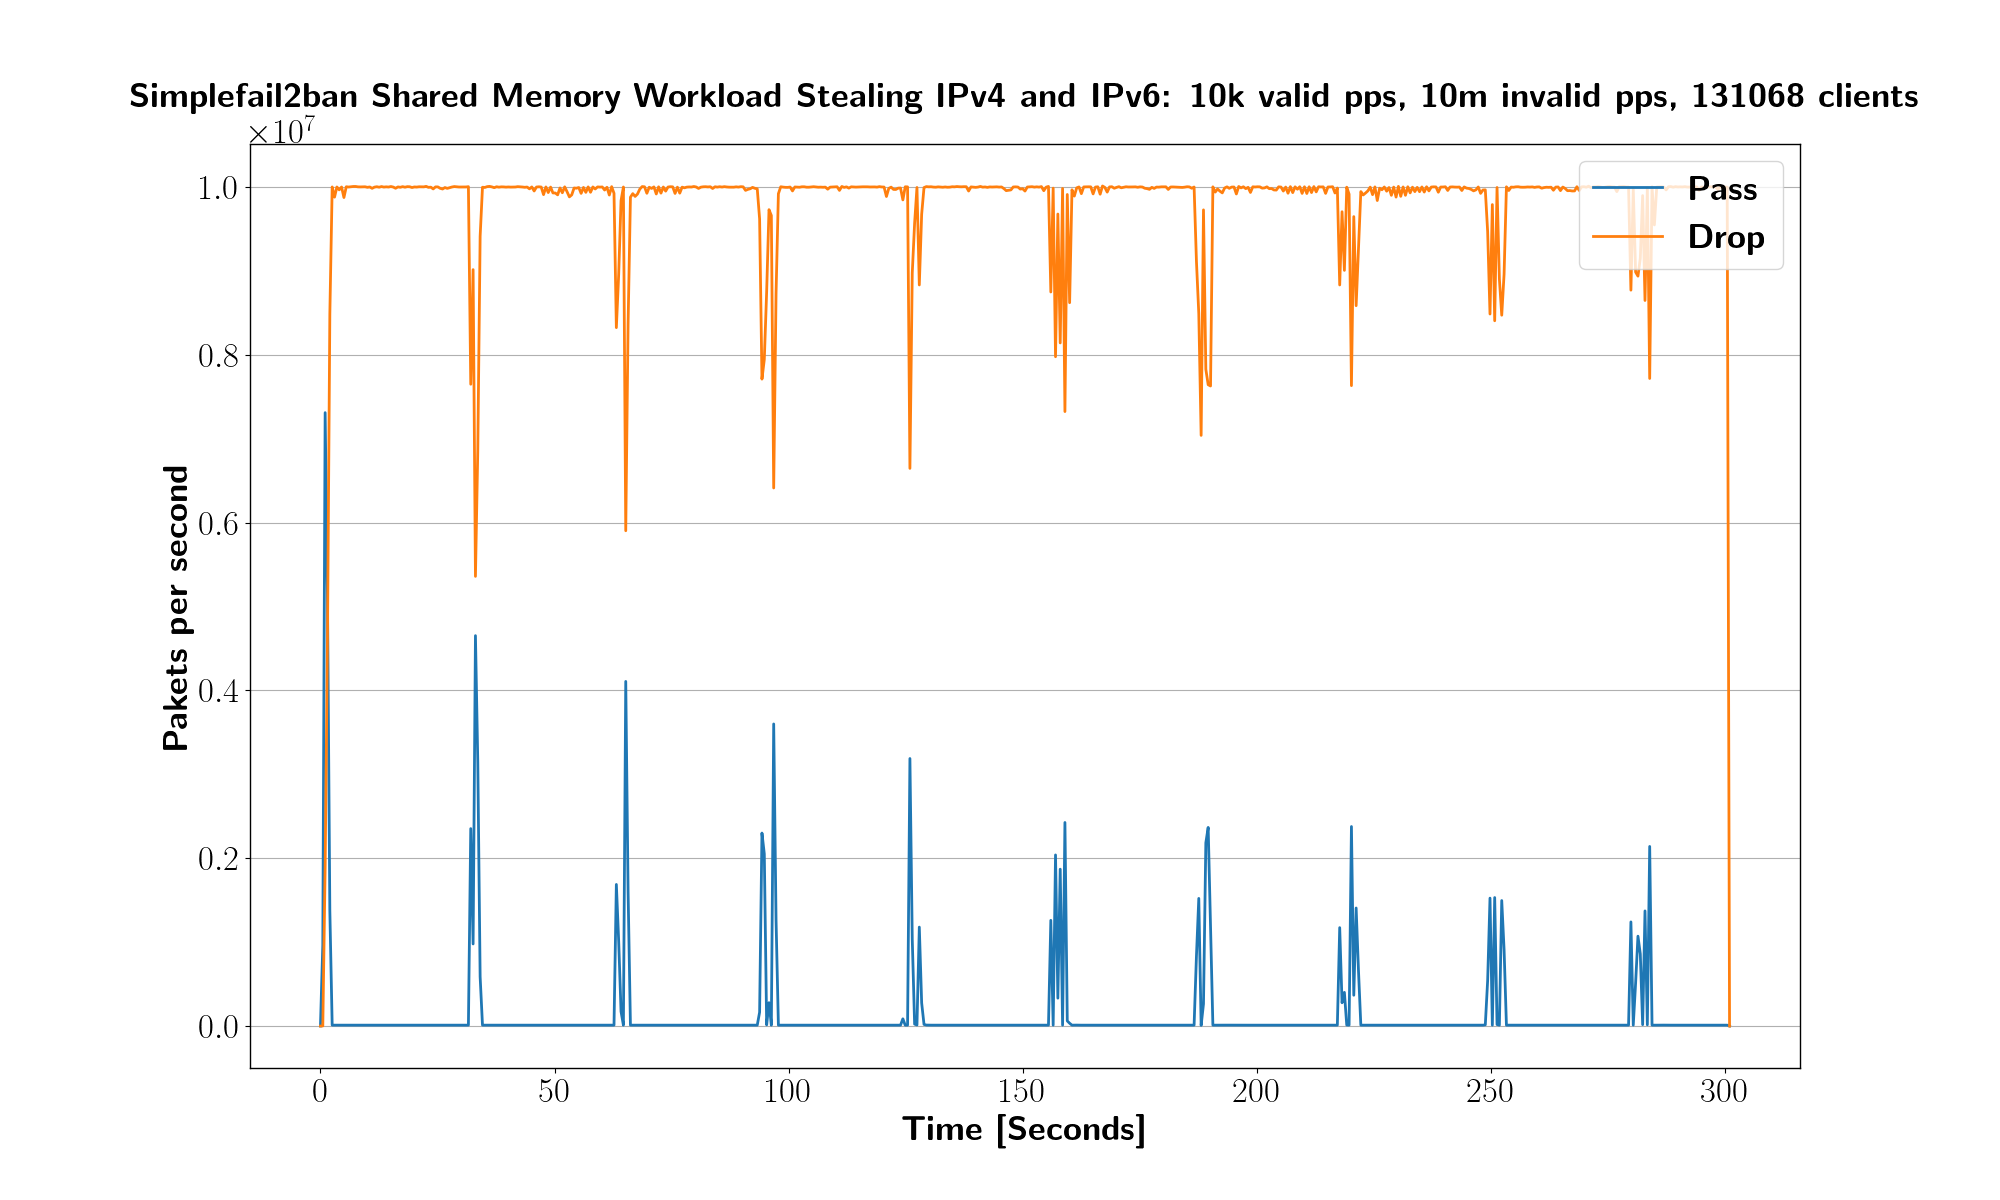
\includegraphics[width=1.2\textwidth]{images/simplefail2ban_shm_ws_ipv46_v10k_iv10m_c131068.png}}
	\end{tabular}
	\begin{tabular}{lllll}
		\toprule
		\textbf{Total packets [$10^6$]} & \textbf{Packets dropped [$10^6$]} & \textbf{Relative drop [\%]} & \textbf{Log messages [$10^6$]} & \textbf{CPU [seconds]} \\ \midrule 
		2991.23 & 2944.56 & 98.67 & 15.28 & 61 \\
		\bottomrule
	\end{tabular}
	\caption[Simplefail2ban, Shared Memory with Workload Sharing]{Some text}
	\label{fig:simplefail2ban:shm:ws}
\end{figure}

Figure \ref{fig:simplefail2ban:shm:ws} presents the results for shared memory Simplefail2ban with the additionally enabled workload stealing feature. Performance does not differ significantly from the baseline measurement. However,
the test scenario is also not ideal for testing workload stealing, as the number of log messages was relatively equal distributed across the buffer segment. Still, about 12\% of all processed log messages were
read via workload stealing. Workload sharing would be expected to have 
larger performance impact, when distribution of messages is highly unequal, as stealing should become more frequent. Creating a specialized test for this scenario could be an objective for future development. 

\pagebreak

\begin{figure}[!h]
	\centering
	\scriptsize
	\begin{tabular}{c}
    	\centerline{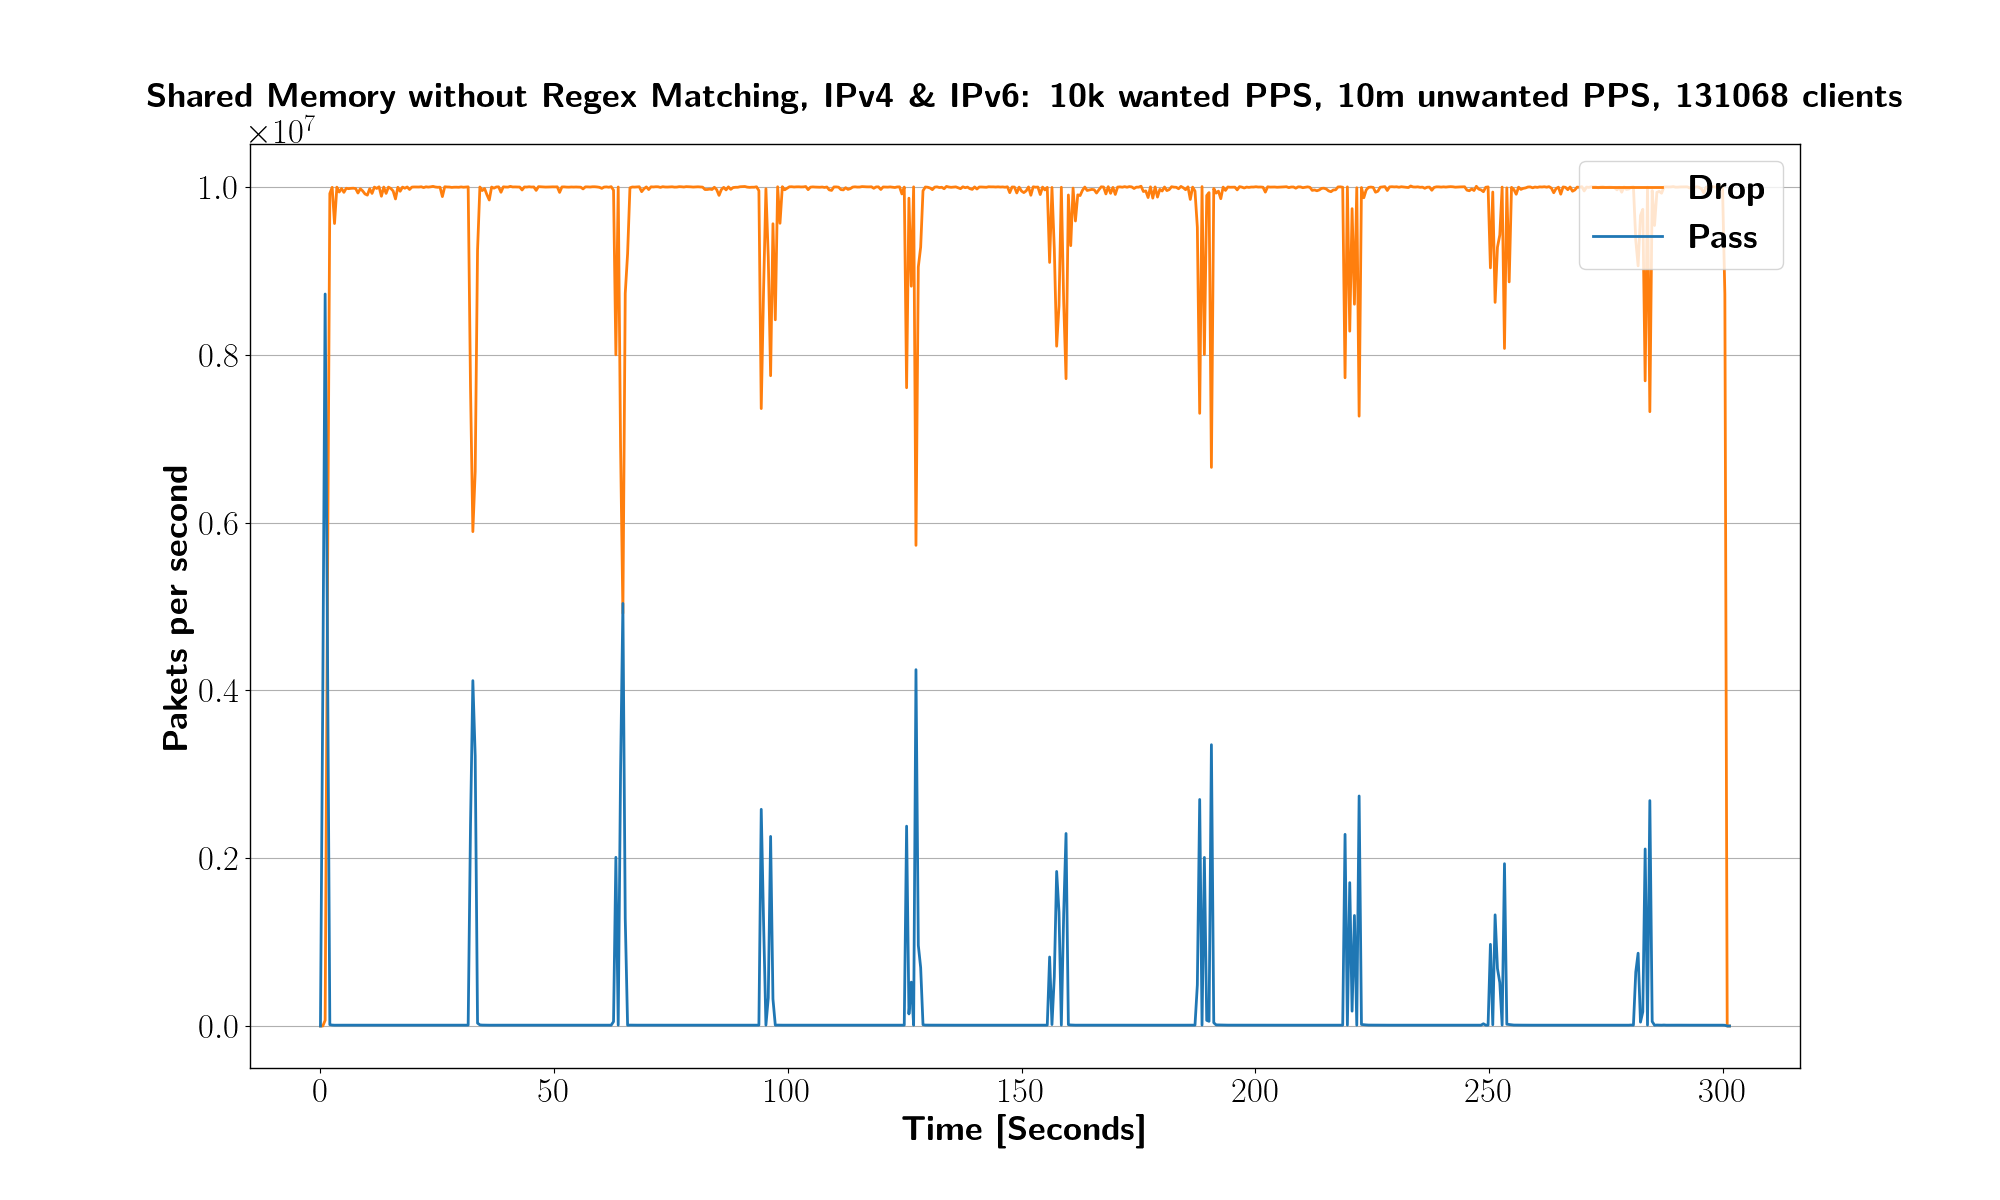
\includegraphics[width=1.2\textwidth]{images/simplefail2ban_shm_nr_ipv46_v10k_iv10m_c131068.png}}
	\end{tabular}
	\begin{tabular}{lllll}
		\toprule
		\textbf{Total packets [$10^6$]} & \textbf{Packets dropped [$10^6$]} & \textbf{Relative drop [\%]} & \textbf{Log messages [$10^6$]} & \textbf{CPU [seconds]} \\ \midrule 
		2989.56 & 2941.9 & 98.63 & 13.29 & 34.04 \\
		\bottomrule
	\end{tabular}
	\caption[Simplefail2ban, Shared Memory without Regex Matching]{Some text}
	\label{fig:simplefail2ban:shm:nr}
\end{figure}

Finally, figure \ref{fig:simplefail2ban:shm:nr} display the result for shared memory Simplefail2ban with directly logged \ac{IP} addresses, instead of \ac{Regex} matching.
This measurement is conducted, to observe the performance impact of the \ac{Regex} matching on the overall performance of Simplefail2ban. The overall performance does not differ
from the baseline measurement. Interestingly, the \ac{CPU} utilization drops by 50\% compared to the baseline. This potentially indicates, that the performance of Simplefail2ban is bottlenecked by 
the speed of the write operations to the \ac{eBPF} maps. Measuring the this performance could be a further objective for future development.   
